\appendix

%\appendixfigures

%\appendixtables 

\section{Spectral fitting and photon path-length derivation}
\label{app:spectral_fit_derivation}

%\subsection{}     %% Appendix A1, A2, etc.


The high-resolution vertical optical depth is computed from layer extinction as
\begin{equation}
\tau_v(\lambda_q)
=
\sum_z
\alpha(\lambda_q,z)\Delta z
+
\tau_{\mathrm{Ray}}(\lambda_q),
\label{eq:vertical_tau_hr}
\end{equation}
where $\alpha$ includes the target absorber and H$_2$O absorption on the ABSCO
grid, and $\tau_{\mathrm{Ray}}$ is the Rayleigh optical depth.


The high-resolution slant optical depth is
\begin{equation}
\mathrm{SOD}(\lambda_q)
=
\left(
\frac{1}{\cos\theta} + \frac{1}{\cos\phi}
\right)
\tau_v(\lambda_q).
\label{eq:hr_sod}
\end{equation}


Because the instrument line shape operates on transmission rather than optical
depth, the channel value used in the fit is
\begin{equation}
\overline{\mathrm{SOD}}_c
=
-\ln
\left[
\frac{
\sum_q R_{cq}\exp\{-\mathrm{SOD}(\lambda_q)\}
}{
\sum_q R_{cq}
}
\right].
\label{eq:discrete_ils_sod}
\end{equation}


The high-resolution solar spectrum is adjusted for Earth--Sun distance and the
solar Doppler stretch before convolution with the instrument line shape:
\begin{equation}
F_{\odot}^{\ast}(\lambda_q)
=
\frac{
F_{\odot}(\lambda_q)
}{
d_{\mathrm{AU}}^2
}
\frac{1}{1+\beta},
\qquad
\lambda_q^{\ast}
=
\lambda_q(1+\beta),
\label{eq:solar_distance_doppler}
\end{equation}
where $d_{\mathrm{AU}}$ is the Earth--Sun distance in astronomical units and
$\beta=v_{\mathrm{solar}}/c$.


The channel solar term is then computed as the ILS-weighted mean,
\begin{equation}
\mathcal{F}_{0,c}^{\mathrm{ILS}}
=
\frac{
\sum_q R_{cq}F_{\odot}^{\ast}(\lambda_q^{\ast})
}{
\sum_q R_{cq}
}.
\label{eq:solar_ils_convolution}
\end{equation}


\begin{equation}
\mathcal{F}_{0,c}
=
m_1
\mathcal{F}_{0,c}^{\mathrm{ILS}}
\frac{1}{\cos\theta},
\qquad
m_1 = 0.5,
\label{eq:effective_solar_normalization}
\end{equation}


\begin{equation}
T_c
=
\frac{\pi I_c}{\mathcal{F}_{0,c}}.
\label{eq:code_transmittance}
\end{equation}






For a photon traveling along the path coordinate $s$ over the total path length $L$, the Beer--Lambert transmittance is
\begin{equation}
T_{\lambda}(L)
=
\exp\left[
-
\int_0^L
\sigma_{\lambda}(s)n(s)
\,\mathrm{d}s
\right]
=
\exp\left[
-
\int_0^L
\alpha_{\lambda}(s)
\,\mathrm{d}s
\right],
\label{eq:beer_lambert_path}
\end{equation}



where $\alpha_{\lambda}(s)=\sigma_{\lambda}(s)n(s)$ is the absorption
coefficient. Averaging over photons with different path lengths gives
\begin{equation}
\bar{T}_{\lambda}
=
\frac{1}{N}
\sum_{i=1}^{N}
\exp\left[
-
\int_0^{L_i}
\alpha_{\lambda,i}(s)
\,\mathrm{d}s
\right].
\label{eq:ensemble_transmittance}
\end{equation}


Under the mean-absorption approximation,
$\alpha_{\lambda,i}(s)\approx\bar{\alpha}_{\lambda}$, so that
\begin{equation}
\bar{T}_{\lambda}
\approx
\frac{1}{N}
\sum_{i=1}^{N}
\exp(-\bar{\alpha}_{\lambda}L_i)
=
\int_0^\infty
p_L(L)
\exp(-\bar{\alpha}_{\lambda}L)
\,\mathrm{d}L .
\label{eq:path_length_laplace_dimensional}
\end{equation}

\begin{equation}
\overline{\mathrm{SOD}}_j
=
-\ln
\left[
\frac{
\sum_q R_j(\lambda_q)
\exp\{-\mathrm{SOD}(\lambda_q)\}
}{
\sum_q R_j(\lambda_q)
}
\right],
\end{equation}

where $j$ indexes the discrete wavelength samples in an OCO-2 band and
$q$ indexes the high-resolution wavelength grid used for the ILS convolution.


Let $\bar{L}$ be the direct geometric slant path and define the dimensionless
path-length enhancement
\begin{equation}
l' = \frac{L}{\bar{L}},
\qquad
\overline{\mathrm{SOD_{c, \lambda}}}
=
\bar{\alpha}_{\lambda}\bar{L}.
\label{eq:path_enhancement_tau}
\end{equation}



The ensemble transmittance can then be written as the Laplace transform of
the path-enhancement distribution:
\begin{equation}
\bar{T}(\overline{\mathrm{SOD}}_c)
=
\int_0^\infty
p(l')
\exp(-\overline{\mathrm{SOD}}_c \, l')
\,\mathrm{d}l' .
\label{eq:path_enhancement_laplace}
\end{equation}


For a Lambertian surface with reflectance $\gamma$,
\begin{equation}
\pi I_c(\lambda)
=
\mathcal{F}_{0,c}(\lambda)\cos\theta\,
\gamma\,
\bar{T}(\overline{\mathrm{SOD}}_{c \, \lambda}),
\label{eq:radiance_lambertian}
\end{equation}



and therefore
\begin{equation}
T(\overline{\mathrm{SOD}}_c)
\equiv
\frac{\pi I_c}{\mathcal{F}_{0,c}\cos\theta}
=
\gamma
\int_0^\infty
p(l')
\exp(-\overline{\mathrm{SOD}}_c \, l')
\,\mathrm{d}l' .
\label{eq:measured_laplace_appendix}
\end{equation}



If $p(l')$ is approximated by a gamma distribution with mean
$\mu_{l'}=\langle l'\rangle$ and shape parameter
$\kappa=\mu_{l'}^2/\operatorname{var}(l')$, then
\begin{equation}
p(l')
=
\frac{(\kappa/\mu_{l'})^{\kappa}}{\Gamma(\kappa)}
l'^{\kappa-1}
\exp\left(-\frac{\kappa}{\mu_{l'}}l'\right),
\qquad
l' \ge 0 .
\label{eq:gamma_path_distribution}
\end{equation}



Its Laplace transform is
\begin{equation}
\int_0^\infty
p(l')\exp(-\overline{\mathrm{SOD}}_c \, l')
\,\mathrm{d}l'
=
\left(
1+\frac{\mu_{l'}}{\kappa}\overline{\mathrm{SOD}}_c
\right)^{-\kappa},
\label{eq:gamma_laplace_transform}
\end{equation}



so the measured transmittance is
\begin{equation}
T(\overline{\mathrm{SOD}}_c)
=
\gamma
\left(
1+\frac{\mu_{l'}}{\kappa}\overline{\mathrm{SOD}}_c
\right)^{-\kappa}.
\label{eq:gamma_transmittance}
\end{equation}



Taking the logarithm gives
\begin{equation}
\ln T(\overline{\mathrm{SOD}}_c)
=
\ln\gamma
-
\kappa
\ln\left(
1+\frac{\mu_{l'}}{\kappa}\overline{\mathrm{SOD}}_c
\right).
\label{eq:log_gamma_transmittance}
\end{equation}


Using the Taylor expansion of the logarithm,
\begin{equation}
\ln T(\overline{\mathrm{SOD}}_c)
=
\ln\gamma
-
\mu_{l'}\overline{\mathrm{SOD}}_c
+
\frac{\mu_{l'}^2}{2\kappa}\overline{\mathrm{SOD}}_c^2
-
\frac{\mu_{l'}^3}{3\kappa^2}\overline{\mathrm{SOD}}_c^3
+
\cdots .
\label{eq:log_gamma_taylor}
\end{equation}



The fitted polynomial is written as
\begin{equation}
\ln T(\overline{\mathrm{SOD}}_c)
=
b
+
\sum_{n=1}^{N}
(-1)^n
\frac{k_n}{n}
\overline{\mathrm{SOD}}_c^n,
\qquad
b=\ln\gamma .
\label{eq:log_polynomial_fit_appendix}
\end{equation}



For the gamma model, matching coefficients gives
\begin{equation}
k_n
=
\frac{\mu_{l'}^{n}}{\kappa^{n-1}},
\qquad
n\ge 1 .
\label{eq:gamma_coefficient_identity}
\end{equation}




Thus
\begin{equation}
k_1=\mu_{l'},
\qquad
k_2=\frac{\mu_{l'}^{2}}{\kappa}
=
\operatorname{var}(l'),
\qquad
\kappa=\frac{k_1^2}{k_2}.
\label{eq:k1_k2_kappa_identity}
\end{equation}

\section{Data provenance, cloud collocation, and target construction}
\label{app:data}





\section{Model architecture, training, and reproducibility}
\label{app:model}



\subsection{Deep-ensemble Member architecture and probabilistic head}

Each of the $M = 5$ ensemble members is a Gaussian-head multilayer perceptron
with two hidden layers (64 and 32 units). Every hidden block applies, in order,
a linear map, layer normalization, a ReLU activation, and 10\% dropout; dropout
is active during training only, so there is no Monte-Carlo dropout at inference
and the ensemble spread alone provides the epistemic uncertainty. For footprint
$i$, member $m$ outputs a predicted mean $\mu_{m,i}$ and a raw second output that is clamped to $[-10, 10]$ and interpreted as the log-variance
$s_{m,i} = \log\sigma_{m,i}^{2}$, giving a per-footprint predictive variance
$\sigma_{m,i}^{2} = \exp(s_{m,i})$.

\subsection{Training loss}

Writing the target as $y_i \equiv \Delta \mathrm{X_{CO2,\,i}^{B11}}$, the standard
Gaussian negative log-likelihood of one footprint is, up to an additive constant,
%
\begin{equation}
  \ell^{\mathrm{NLL}}_{m,i}
  = \frac{1}{2}\left[\,s_{m,i}
  + \frac{(y_i-\mu_{m,i})^{2}}{\sigma_{m,i}^{2}}\,\right].
  \label{eq:gauss-nll}
\end{equation}
%
Because this loss down-weights high-variance footprints, the mean is poorly
fitted exactly in the near-cloud regime where $\sigma_{m,i}^{2}$ is large. We
therefore train the members with the $\beta$-NLL loss of
\citet{seitzer2022pitfalls}, which multiplies each footprint's NLL by a
stop-gradient function of its own predicted variance,
%
\begin{equation}
  \ell^{\beta\text{-}\mathrm{NLL}}_{m,i}
  = \bigl\lfloor\sigma_{m,i}^{2}\bigr\rfloor_{\mathrm{sg}}^{\,\beta}\;
  \ell^{\mathrm{NLL}}_{m,i},
  \qquad \beta = 0.5,
  \label{eq:beta-nll}
\end{equation}
%
where $\lfloor\cdot\rfloor_{\mathrm{sg}}$ denotes a stop-gradient (the weight is
treated as a constant during backpropagation). Here $\beta = 0$ recovers the
plain NLL of Eq.~\eqref{eq:gauss-nll} and $\beta = 1$ recovers a
mean-squared-error weighting of the mean; the production choice $\beta = 0.5$
restores the mean-fitting gradient in the high-variance near-cloud footprints
while keeping a calibrated variance. The member loss is the average of
Eq.~\eqref{eq:beta-nll} over the training footprints.

\subsection{Ensemble aggregation}

The five members differ only in their random seed (member $m$ uses seed
$s_0 + m$), so their predictions decorrelate and the ensemble spread provides
the epistemic uncertainty. The per-member means and variances are combined as a
Gaussian mixture,
%
\begin{equation}
  \mu^{*}_i = \frac{1}{M}\sum_{m=1}^{M}\mu_{m,i},
  \qquad
  \sigma^{*2}_i
  = \underbrace{\frac{1}{M}\sum_{m=1}^{M}\sigma_{m,i}^{2}}_{\text{aleatoric}}
  + \underbrace{\frac{1}{M}\sum_{m=1}^{M}\mu_{m,i}^{2} - \mu^{*2}_i}_{\text{epistemic}},
  \label{eq:mixture}
\end{equation}
%
which is the law of total variance: the first term is the mean aleatoric
variance predicted by the heads and the second is the between-member (epistemic)
variance. The ensemble mean $\mu^{*}_i$ is the point correction applied to each
footprint.

\subsection{Optimization and leakage control}

Each member is optimized with AdamW (learning rate $10^{-3}$, weight decay
$10^{-4}$) under a one-cycle learning-rate schedule with gradient-norm clipping
at $1.0$, a batch size of $4096$, and up to $500$ epochs. Training is stopped
early on the held-out calibration block (patience of $50$ epochs), and the
checkpoint with the lowest calibration loss is kept; the calibration block is
carved from the training dates and never overlaps the held-out fold or the
validation references. The calibration block is also used to recalibrate the
Mondrian conformal intervals, which are binned by predicted-anomaly deciles.
Feature scaling and any profile-EOF transforms are fitted on the proper-training
partition only. Table~\ref{tab:hyperparams} collects the full configuration.

\begin{table}[t]
\centering
\caption{DE-MLP architecture and training configuration (production settings).}
\label{tab:hyperparams}
\begin{tabular}{@{}ll@{}}
\toprule
Component & Setting \\
\midrule
Ensemble members $M$        & 5 (seeds $s_0 + m$) \\
Hidden layers               & 64, 32 \\
Hidden block                & Linear $\to$ LayerNorm $\to$ ReLU $\to$ Dropout(0.1) \\
Output head                 & Linear $\to$ 2 (mean, log-variance) \\
Log-variance clamp          & $[-10, 10]$ \\
Loss                        & $\beta$-NLL, $\beta = 0.5$ \\
Optimizer                   & AdamW \\
Learning rate (max)         & $10^{-3}$ \\
Weight decay                & $10^{-4}$ \\
LR schedule                 & one-cycle (\texttt{pct\_start} 0.05, div 25, final div 1000) \\
Gradient clipping           & 1.0 (max norm) \\
Batch size                  & 4096 \\
Maximum epochs              & 500 \\
Early stopping              & patience 50, on the calibration block \\
Calibration fraction        & 0.15 of the training dates \\
Conformal intervals         & Mondrian, 10 predicted-anomaly decile bins \\
\bottomrule
\end{tabular}
\end{table}


\subsection{Loss function for \emph{Ridge} and \emph{XGBoost} models}

The LR and XGBoost models are trained with the following objectives, all on the same target $y_i \equiv \Delta \mathrm{X_{CO2,\,i}^{B11}}$ and the same
train-only-standardized features $\mathbf{x}_i$.

\subsubsection*{Ridge} 
A linear predictor $\hat{y}_i = \mathbf{x}_i^{\top}\bm{\beta}$
trained by $\ell_2$-penalized least squares,
%
\begin{equation}
  \mathcal{L}_{\mathrm{Ridge}}(\bm{\beta})
  = \sum_i \bigl(y_i - \mathbf{x}_i^{\top}\bm{\beta}\bigr)^{2}
  + \alpha\,\lVert\bm{\beta}\rVert_{2}^{2},
  \label{eq:ridge}
\end{equation}
%
with the penalty $\alpha$ selected from $\{0.1, 1, 10, 100\}$ by lowest RMSE on
the calibration block.

\subsection*{XGBoost} 
A gradient-boosted tree ensemble
$\hat{y}_i = \sum_{t} f_t(\mathbf{x}_i)$ minimizing a regularized squared-error
objective,
%
\begin{equation}
  \mathcal{L}_{\mathrm{XGB}}
  = \sum_i \bigl(y_i - \hat{y}_i\bigr)^{2}
  + \sum_t \Omega(f_t),
  \qquad
  \Omega(f) = \tfrac{1}{2}\lambda\lVert w \rVert_{2}^{2},
  \label{eq:xgb}
\end{equation}
%
where $\Omega$ penalizes the leaf weights $w$ ($\lambda = 1$) and the number of
boosting rounds is early-stopped on the calibration block (maximum tree depth
$6$).

% \paragraph{DE-MLP.} Each of the $M = 5$ members minimizes the mean $\beta$-NLL
% loss of Eq.~\eqref{eq:beta-nll}; the ensemble prediction follows
% Eq.~\eqref{eq:mixture}.


\subsection{Model Predictors}

% Auto-generated by make_appendix_c_figures.py — do not hand-edit.
\begingroup\footnotesize
\begin{longtable}{lccp{0.50\linewidth}}
\caption{Full predictor inventory of the per-surface correction models (ocean: 56 inputs; land: 67), generated from the feature pipeline source. All quantities are per-sounding OCO-2 L2 Lite columns except the spectral path-length block (fitted from the L1B spectrum, Sect.~3.2) and the profile-EOF block (fold-fitted PCA of the Lite meteorology/prior profiles). Sfc: which surface model uses the feature. Transform: RS $=$ robust--standard scaling (median/IQR, then standardization), log1p applied first where marked; SS $=$ block-own standard scaler; both fitted on the training split only. Cloud distance is not an input.}
\label{tab:predictor-inventory}\\
\tophline
Feature & Sfc & Transform & Description \\
\middlehline
\endfirsthead
\multicolumn{4}{l}{\textit{(continued)}}\\
\tophline
Feature & Sfc & Transform & Description \\
\middlehline
\endhead
\bottomhline
\endfoot
\bottomhline
\multicolumn{4}{p{0.9\linewidth}}{\footnotesize The three named ablation groups of Table~2 map exactly onto the groups above: $-$xco2 drops the retrieval-state row, $-$spec the spectral path-length block, $-$contam the contamination-indicator block.}\\
\endlastfoot
\multicolumn{4}{l}{\textit{Retrieval state}} \\
\texttt{xco2\_raw\_minus\_apriori} & O$+$L & RS & Retrieved (pre-bias-correction) XCO$_2$ minus prior XCO$_2$ (ppm) \\
\middlehline
\multicolumn{4}{l}{\textit{Spectral path-length}} \\
\texttt{exp\_o2a\_intercept} & O$+$L & RS & O$_2$A continuum reflectance (exponential of the cumulant-fit intercept) \\
\texttt{o2a\_exp\_intercept-alb} & O$+$L & RS & O$_2$A continuum reflectance minus retrieved O$_2$A albedo \\
\texttt{o2a\_k1\_nosg} & O$+$L & RS & O$_2$A mean relative photon path $\langle l'\rangle$ (this work, Sect.~3.2) \\
\texttt{o2a\_k2\_nosg} & O$+$L & RS & O$_2$A photon-path variance $\mathrm{var}(l')$ \\
\texttt{wco2\_k1\_nosg} & O$+$L & RS & WCO$_2$ $\langle l'\rangle$ \\
\texttt{wco2\_k2\_nosg} & O$+$L & RS & WCO$_2$ $\mathrm{var}(l')$ \\
\texttt{wco2\_k3\_nosg} & O$+$L & RS & WCO$_2$ third-order path-length cumulant \\
\texttt{sco2\_k1\_nosg} & O$+$L & RS & SCO$_2$ $\langle l'\rangle$ \\
\texttt{sco2\_k2\_nosg} & O$+$L & RS & SCO$_2$ $\mathrm{var}(l')$ \\
\texttt{wco2\_exp\_intercept-alb} & L & RS & WCO$_2$ continuum reflectance minus retrieved WCO$_2$ albedo \\
\middlehline
\multicolumn{4}{l}{\textit{Geometry \& L1B diagnostics}} \\
\texttt{fp\_area\_km2} & O$+$L & log1p$+$RS & Footprint area (km$^2$) \\
\texttt{cos\_glint\_angle} & O & RS & Cosine of the glint angle \\
\texttt{h2o\_ratio\_bc} & O$+$L & RS & IDP H$_2$O band-ratio cloud-screen diagnostic (bias-corrected) \\
\texttt{csnr\_sco2} & O & RS & Continuum signal-to-noise ratio, SCO$_2$ band \\
\texttt{pol\_ang\_rad} & O$+$L & RS & Polarization angle (rad) \\
\texttt{s31} & O$+$L & RS & Band signal ratio SCO$_2$/O$_2$A \\
\texttt{1\_over\_cos\_sza} & L & RS & Solar air-mass factor $1/\cos(\mathrm{SZA})$ \\
\texttt{1\_over\_cos\_vza} & L & RS & Viewing air-mass factor $1/\cos(\mathrm{VZA})$ \\
\texttt{sin\_raa} & L & RS & Sine of the relative azimuth angle \\
\texttt{co2\_ratio\_bc} & L & RS & IDP CO$_2$ band-ratio cloud-screen diagnostic (bias-corrected) \\
\texttt{csnr\_o2a} & L & RS & Continuum signal-to-noise ratio, O$_2$A band \\
\texttt{h\_cont\_o2a} & L & RS & O$_2$A continuum-radiance variability across adjacent soundings (per-sounding preprocessor value) \\
\texttt{h\_cont\_sco2} & L & RS & SCO$_2$ continuum-radiance variability across adjacent soundings \\
\middlehline
\multicolumn{4}{l}{\textit{Meteorology, surface \& aerosol}} \\
\texttt{log\_P} & O$+$L & RS & Log of retrieved surface pressure \\
\texttt{dp\_psfc\_prior\_ratio} & O$+$L & RS & Retrieved-minus-prior surface pressure, relative to the prior \\
\texttt{h2o\_scale} & O$+$L & RS & Retrieved H$_2$O-profile scale factor \\
\texttt{delT} & O$+$L & RS & Retrieved temperature-profile offset (K) \\
\texttt{co2\_grad\_del} & O$+$L & RS & Change in the retrieved CO$_2$ vertical gradient relative to the prior \\
\texttt{aod\_dust} & O$+$L & log1p$+$RS & Retrieved dust aerosol optical depth \\
\texttt{aod\_oc} & O$+$L & log1p$+$RS & Retrieved organic-carbon aerosol optical depth \\
\texttt{aod\_seasalt} & O$+$L & log1p$+$RS & Retrieved sea-salt aerosol optical depth \\
\texttt{aod\_strataer} & O$+$L & log1p$+$RS & Retrieved stratospheric-aerosol optical depth \\
\texttt{aod\_sulfate} & O$+$L & log1p$+$RS & Retrieved sulfate aerosol optical depth \\
\texttt{tcwv} & O$+$L & RS & Total column water vapour \\
\middlehline
\multicolumn{4}{l}{\textit{Contamination indicators}} \\
\texttt{max\_declock\_wco2} & O & RS & Maximum WCO$_2$ declocking correction (detector diagnostic) \\
\texttt{aod\_water} & O$+$L & log1p$+$RS & Retrieved water-cloud optical depth \\
\texttt{dp\_abp} & O$+$L & RS & A-band-preprocessor surface-pressure difference (cloud screen) \\
\texttt{h\_cont\_wco2} & O$+$L & RS & WCO$_2$ continuum-radiance variability across adjacent soundings \\
\texttt{t700} & O$+$L & RS & Temperature at 700\,hPa (K) \\
\texttt{water\_height} & O$+$L & RS & Retrieved water-cloud layer height \\
\texttt{alb\_sco2\_over\_wco2} & O$+$L & RS & Retrieved albedo ratio SCO$_2$/WCO$_2$ \\
\texttt{dpfrac} & L & RS & Fractional retrieved-minus-prior surface-pressure difference \\
\texttt{fs\_rel\_0} & L & RS & Relative fluorescence signal (clamped $\geq 0$) \\
\texttt{dust\_height} & L & RS & Retrieved dust layer height \\
\texttt{aod\_ice} & L & log1p$+$RS & Retrieved ice-cloud optical depth \\
\texttt{ice\_height} & L & RS & Retrieved ice-cloud layer height \\
\texttt{alt\_std} & L & RS & Std.\ dev.\ of surface altitude within the footprint (roughness) \\
\middlehline
\multicolumn{4}{l}{\textit{Footprint}} \\
\texttt{fp\_0}\,\ldots\,\texttt{fp\_7} & O$+$L & none & Footprint-index one-hot (8 across-track positions) \\
\middlehline
\multicolumn{4}{l}{\textit{Profile EOFs (appended block)}} \\
\texttt{t\_pc01}--\texttt{t\_pc04} & O$+$L & SS & Temperature-profile EOF scores ($\sigma$-grid, per surface) \\
\texttt{q\_pc01}--\texttt{q\_pc04} & O$+$L & SS & Specific-humidity EOF scores (log-compressed $\sigma$-grid) \\
\texttt{co2prior\_pc01}--\texttt{co2prior\_pc04} & O$+$L & SS & Shape-normalized prior-CO$_2$-profile EOF scores \\
\texttt{tropopause\_sigma} & O$+$L & SS & Tropopause pressure in $\sigma$ coordinate \\
\texttt{tropopause\_temp} & O$+$L & SS & Tropopause temperature (K) \\
\end{longtable}
\endgroup




\subsection{Data split}



%
\begin{figure}[t]
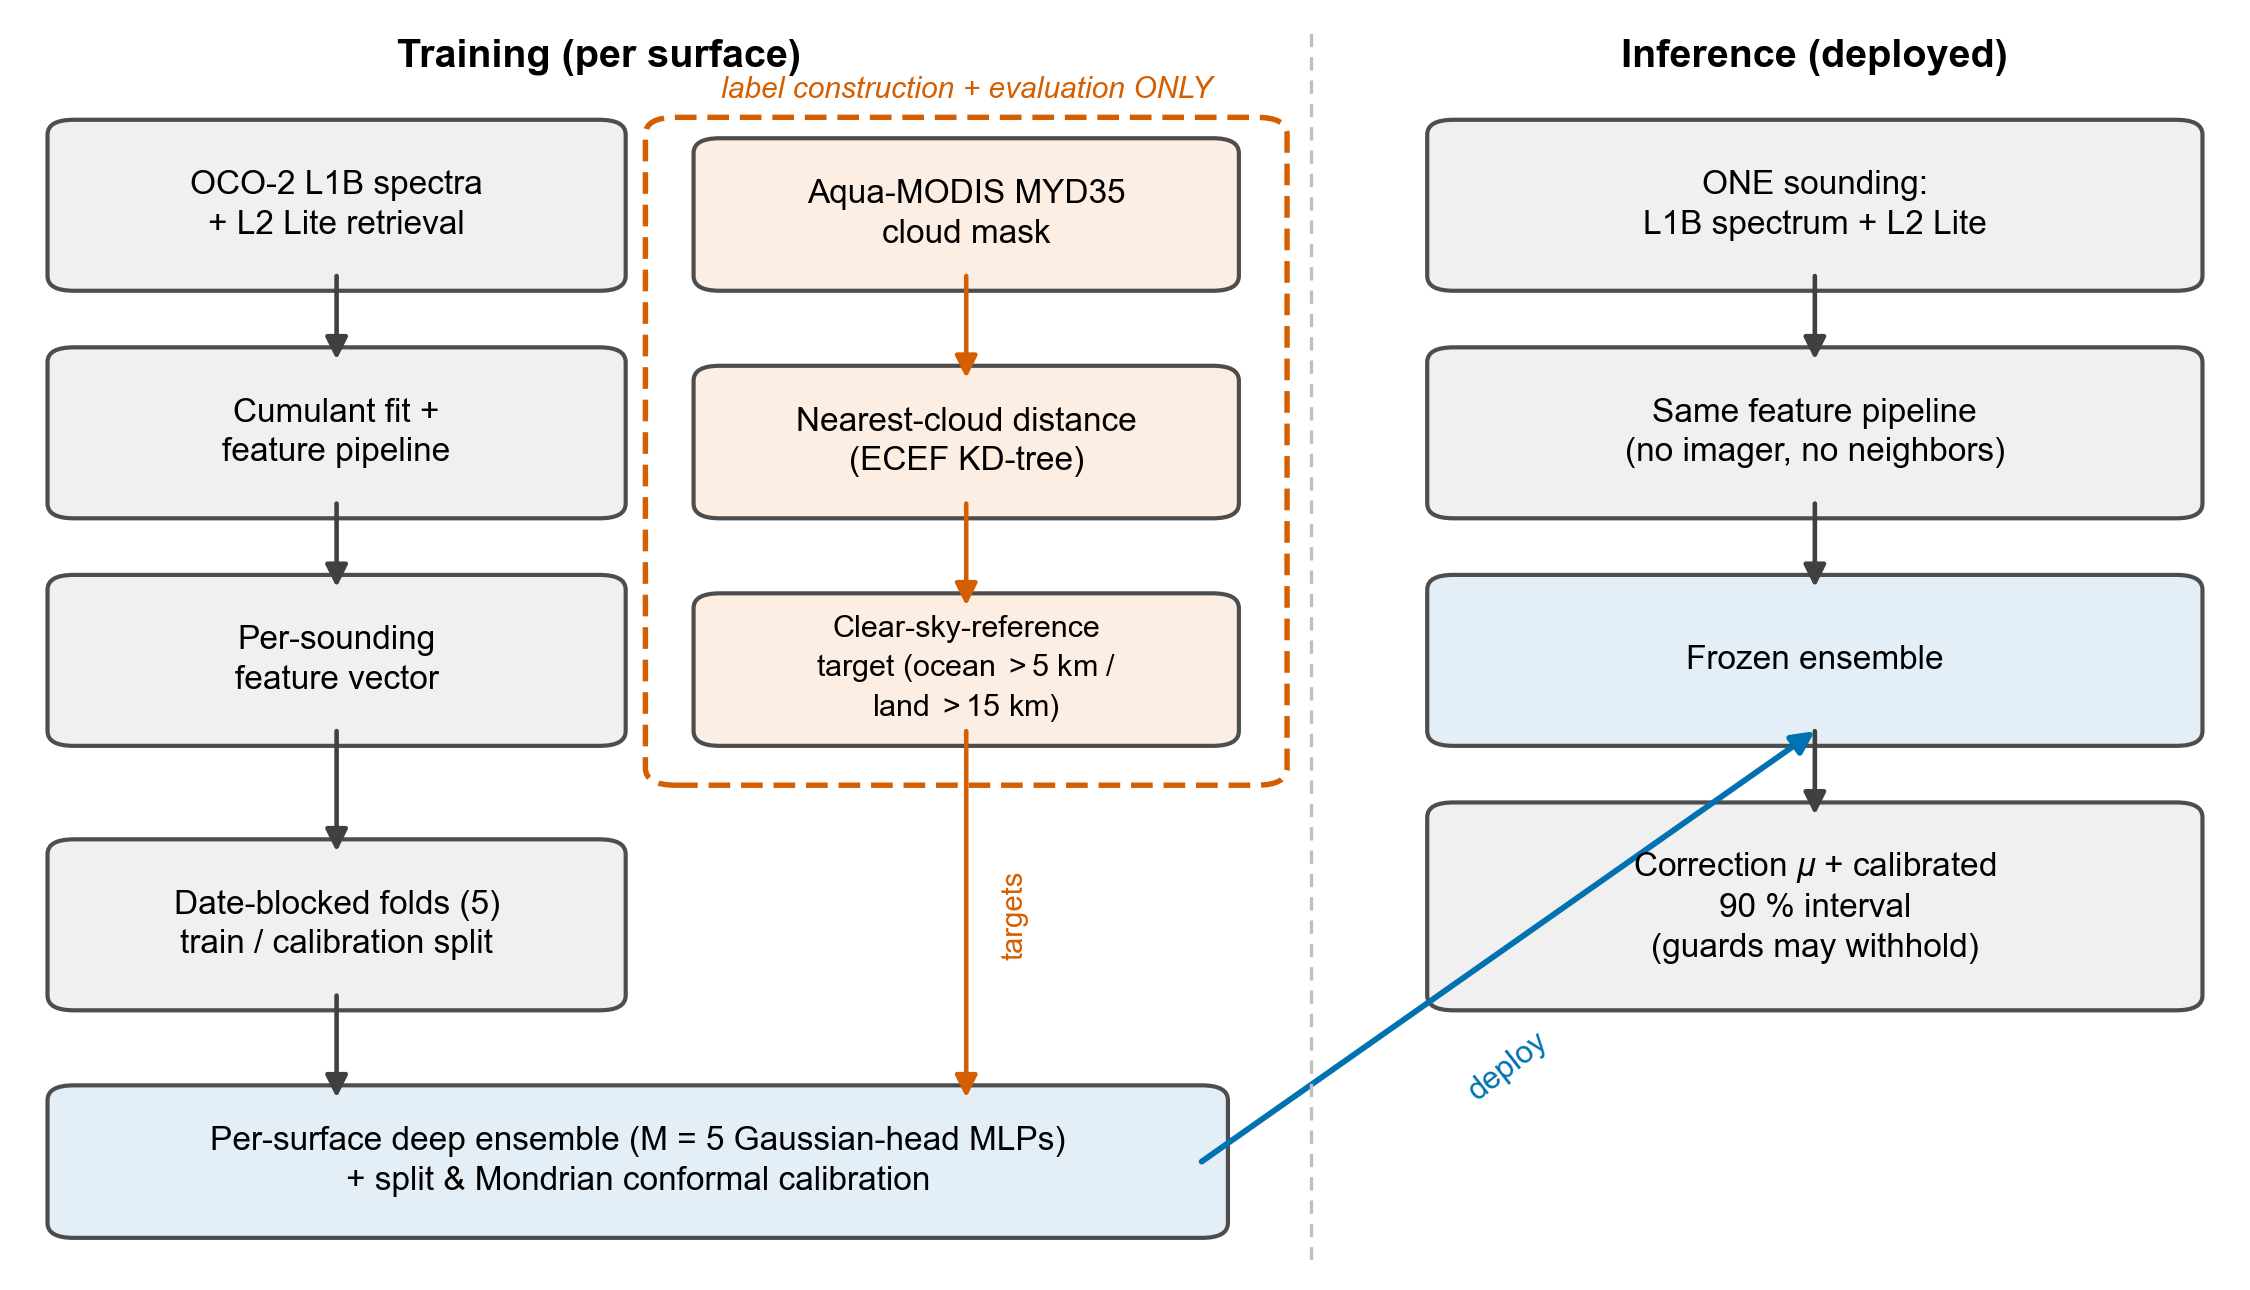
\includegraphics[width=\textwidth]{figures/figC1_dataflow.png}
\caption{Scheme of the data flow from training to inference/bias correction.}
\label{fig:train_infer_flow}
\end{figure}
%

\begin{figure}[t]
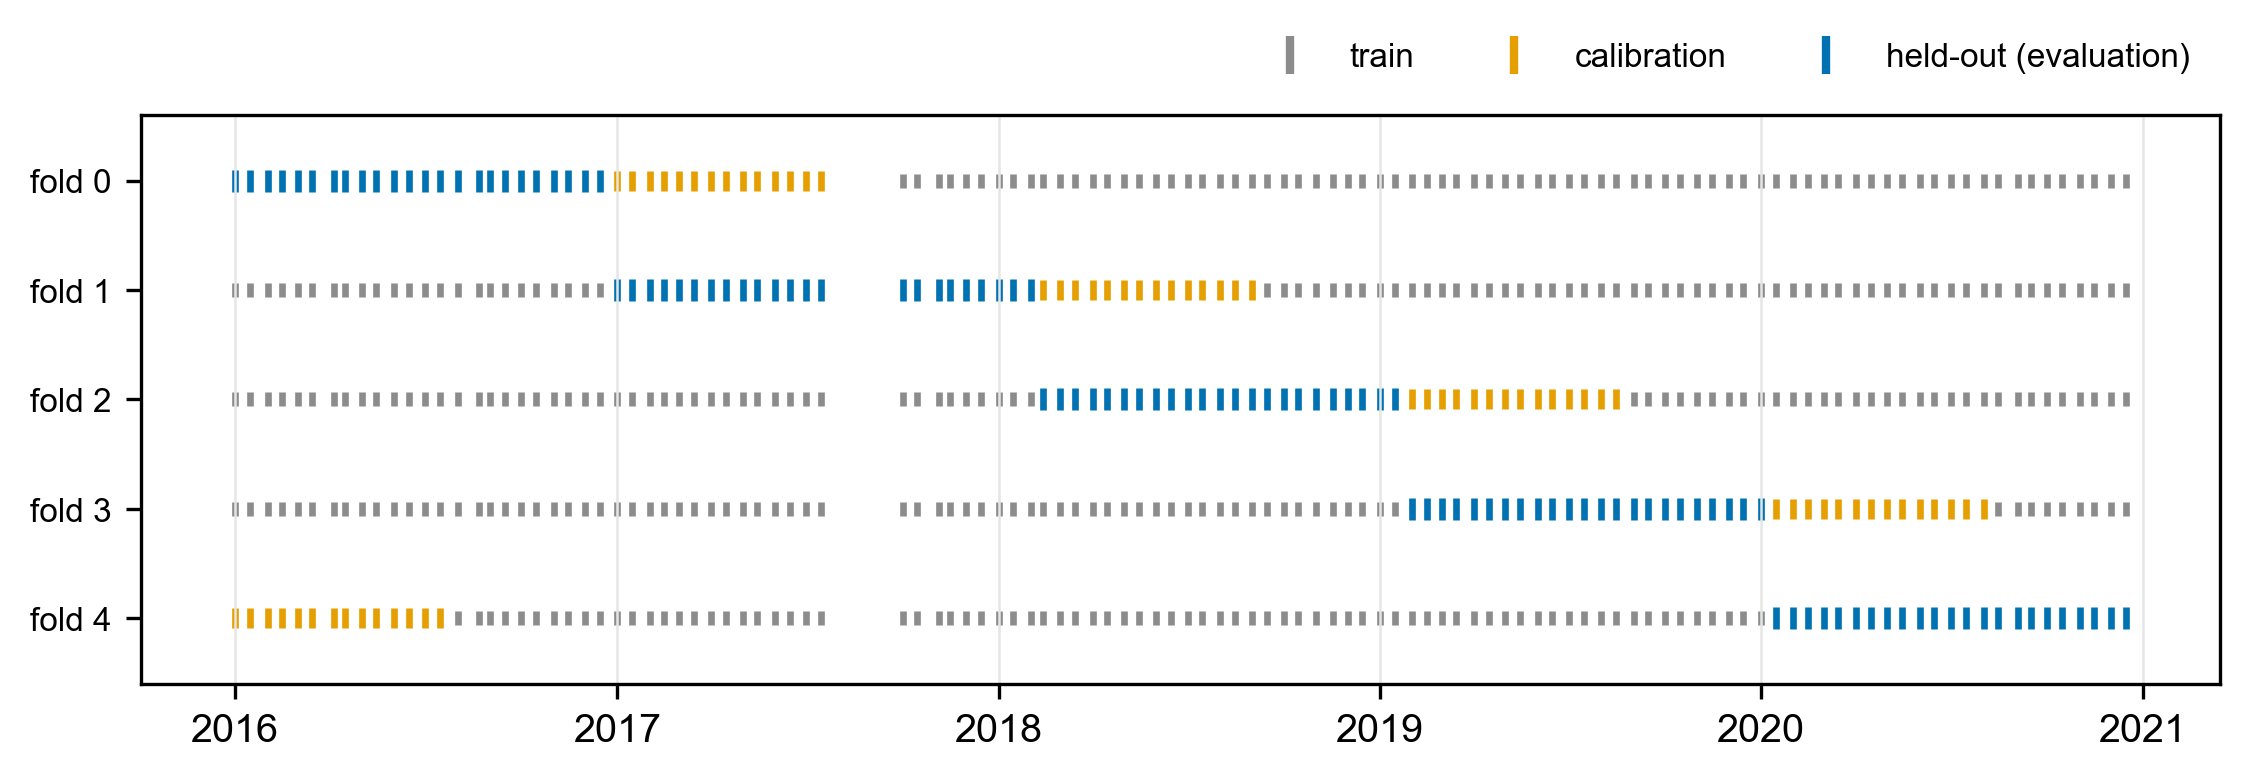
\includegraphics[width=\textwidth]{figures/figC2_fold_timeline.png}
\caption{Five-fold block-rotation cross-validation design over the 116
training and analysis dates. Each fold holds out one contiguous block of dates as
the test subset, and the remaining dates are divided into the proper-training and
the calibration subsets.}
\label{fig:5fold_illustration}
\end{figure}
%



\subsection{Model comparison}
\label{app:model_compare}



\begin{figure}[t]
\centering
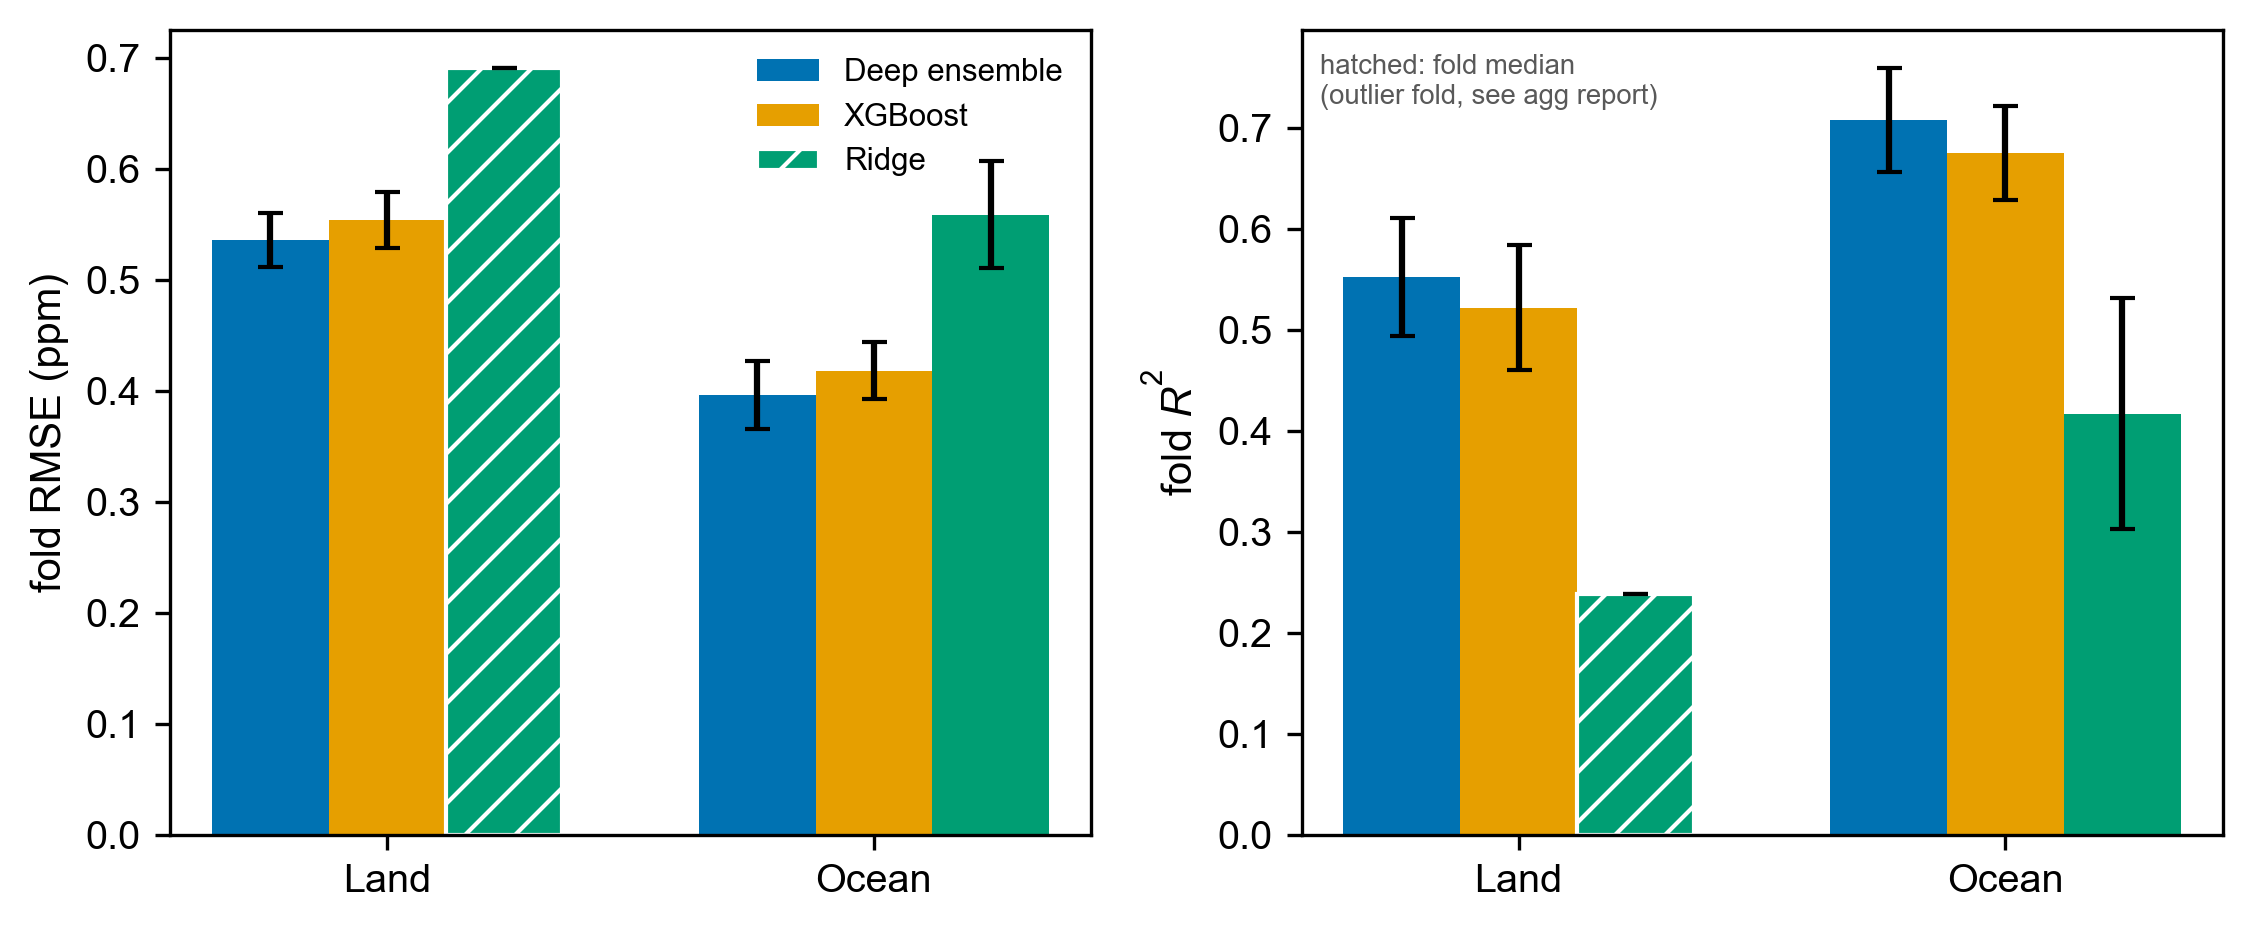
\includegraphics[width=0.8\textwidth]{figures/figC5_cv_model_comparison.png}
\caption{Date-blocked five-fold cross-validation of the anomaly target: held-out fold RMSE (left) and $R^2$ (right), mean ± std over folds, for the deep ensemble, XGBoost, and ridge baselines per surface. Ridge predictions pass the production output guard (Table C5 note).}
\label{fig:model_cv_compare}
\end{figure}



% Auto-generated by make_appendix_c_figures.py — do not hand-edit.
\begingroup\small
\begin{longtable}{lp{0.60\linewidth}}
\caption{Production training configuration of the per-surface deep ensembles, read from the ten fold run manifests (identical across surfaces and folds by assertion).}
\label{tab:training-config}\\
\tophline
Setting & Value \\
\middlehline
\endfirsthead
\multicolumn{2}{l}{\textit{(continued)}}\\
\tophline
Setting & Value \\
\middlehline
\endhead
\bottomhline
\endfoot
\bottomhline
\endlastfoot
Member architecture & MLP $n\rightarrow$64$\rightarrow$32$\rightarrow(\mu, \log\sigma^2)$ Gaussian heads \\
Normalization / dropout & layer normalization / 0.1 \\
Loss & $\beta$-NLL, $\beta = 1$ \\
Members per fold $M$ & 5 \\
Folds & 5, contiguous date blocks (Fig.~C2); pooled inference ensemble $5\times M = 25$ \\
Calibration split & 0.15 of training dates (date-blocked; early stopping and conformal calibration) \\
Optimizer & AdamW, lr 0.001, weight decay 0.0001 \\
Schedule & OneCycle (pct\_start 0.05, div 25, final div 1000) \\
Batch size / max epochs & 8192 / 500 (early stop, patience 50, best-validation checkpoint) \\
Gradient clip / seed & 1 / 42 \\
Feature set & \texttt{full} $+$ profile-EOF block (fold-fitted PCA) \\
Feature scaling & robust--standard scaler; log1p on AODs and footprint area; fitted on the training split only \\
Uncertainty calibration & split $+$ Mondrian conformal (cloud-distance bins), 90\,\% intervals \\
\end{longtable}
\endgroup


% Auto-generated by make_appendix_c_figures.py — do not hand-edit.
\begin{table}[t]
\caption{Fold-level sample sizes and held-out performance of the production deep ensemble. Dates: training/calibration/held-out date counts of the shared date-blocked fold structure (Fig.~C2); $n$: held-out soundings; RMSE (ppm) and $R^2$ against the anomaly target; cov$_{90}$ and width (ppm): empirical coverage and mean width of the Mondrian-conformal 90\,\% intervals.}
\label{tab:fold-sizes-metrics}
\small
\begin{tabular}{lcrrrrr}
\tophline
Fold & Dates (tr/cal/held) & $n$ & RMSE & $R^2$ & cov$_{90}$ & width \\
\middlehline
\multicolumn{7}{l}{\textit{Ocean (r05)}} \\
fold 0 & 78/14/24 & 1\,592\,441 & 0.449 & 0.619 & 0.945 & 1.74 \\
fold 1 & 79/14/23 & 1\,635\,886 & 0.397 & 0.710 & 0.945 & 1.53 \\
fold 2 & 79/14/23 & 1\,758\,400 & 0.375 & 0.747 & 0.955 & 1.57 \\
fold 3 & 79/14/23 & 1\,521\,313 & 0.380 & 0.727 & 0.956 & 1.57 \\
fold 4 & 79/14/23 & 1\,340\,722 & 0.381 & 0.735 & 0.978 & 1.90 \\
\middlehline
\multicolumn{7}{l}{\textit{Land (r15)}} \\
fold 0 & 78/14/24 & 803\,684 & 0.577 & 0.470 & 0.915 & 1.91 \\
fold 1 & 79/14/23 & 739\,808 & 0.537 & 0.577 & 0.898 & 1.68 \\
fold 2 & 79/14/23 & 755\,293 & 0.534 & 0.539 & 0.899 & 1.68 \\
fold 3 & 79/14/23 & 752\,939 & 0.519 & 0.628 & 0.908 & 1.70 \\
fold 4 & 79/14/23 & 792\,948 & 0.515 & 0.547 & 0.913 & 1.70 \\
\bottomhline
\end{tabular}
\end{table}


% Auto-generated by make_appendix_c_figures.py — do not hand-edit.
\begin{table*}[t]
\caption{Training-date manifests and evaluation-date disjointness. The 116 model dates (training, calibration, and held-out roles pooled over all five folds; identical for both surfaces) are compared against every independent evaluation set; the intersection column is computed from the per-run \texttt{training\_dates.json} manifests at table-generation time and enforced programmatically by the leakage guard in every evaluation builder.}
\label{tab:manifest-verification}
\small
\begin{tabular}{lrrcr}
\tophline
Set & Cases & Unique dates & Date range & $\cap$ model dates \\
\middlehline
Training $+$ calibration $+$ held (all folds) & — & 116 & 2016-01-01 -- 2020-12-15 & — \\
\middlehline
TCCON (A-train era) & 75 & 51 & 2014-12-03 -- 2021-12-29 & 0 \\
TCCON (drift era) & 21 & 21 & 2023-01-23 -- 2024-12-02 & 0 \\
ATom pseudo-columns & 8 & 8 & 2017-01-26 -- 2018-05-12 & 0 \\
Shipborne EM27/SUN & 4 & 4 & 2019-06-09 -- 2021-03-15 & 0 \\
\bottomhline
\end{tabular}
\end{table*}


% Auto-generated by make_appendix_c_figures.py — do not hand-edit.
\begin{table}[t]
\caption{Date-blocked five-fold cross-validation of the anomaly target: held-out fold RMSE (ppm) and $R^2$ (mean $\pm$ std over folds) for the deep ensemble (DE), XGBoost, and ridge baselines, per surface.}
\label{tab:cv-model-comparison}
\begin{tabular}{llrr}
\tophline
Surface & Model & RMSE (ppm) & $R^2$ \\
\middlehline
Ocean & DE & $0.396 \pm 0.027$ & $0.708 \pm 0.046$ \\
Ocean & XGBoost & $0.418 \pm 0.023$ & $0.675 \pm 0.042$ \\
Ocean & Ridge$^{*}$ & $0.537 \pm 0.023$ & $0.464 \pm 0.054$ \\
\middlehline
Land & DE & $0.536 \pm 0.022$ & $0.552 \pm 0.052$ \\
Land & XGBoost & $0.554 \pm 0.023$ & $0.522 \pm 0.055$ \\
Land & Ridge$^{*}$ & $0.673 \pm 0.021$ & $0.299 \pm 0.033$ \\
\bottomhline
\end{tabular}
\belowtable{$^{*}$Ridge predictions pass the production output guard (correction withheld where $|\mu| > 25$\,ppm), which the deployed chain applies to every model; it triggers on 18 of the $\sim$11.6\,M ridge held-out footprints — dominated by a single out-of-domain footprint whose unbounded linear extrapolation reaches $|\mu| \sim 10^{6}$\,ppm — and is not applied to the bounded DE/XGBoost outputs (max $|\mu| < 32$\,ppm).}
\end{table}


% Auto-generated by make_appendix_c_figures.py — do not hand-edit.
\begin{table}[t]
\caption{Fold-resolved held-out metrics (RMSE in ppm, $R^2$) for the deep ensemble, XGBoost, and ridge baselines under the shared date-blocked folds. Ridge values apply the production output guard of Table~C5.}
\label{tab:fold-resolved-baselines}
\small
\begin{tabular}{lrrrrrr}
\tophline
& \multicolumn{2}{c}{DE} & \multicolumn{2}{c}{XGBoost} & \multicolumn{2}{c}{Ridge} \\
Fold & RMSE & $R^2$ & RMSE & $R^2$ & RMSE & $R^2$ \\
\middlehline
\multicolumn{7}{l}{\textit{Ocean (r05)}} \\
fold 0 & 0.449 & 0.619 & 0.461 & 0.599 & 0.583 & 0.358 \\
fold 1 & 0.397 & 0.710 & 0.420 & 0.674 & 0.524 & 0.492 \\
fold 2 & 0.375 & 0.747 & 0.392 & 0.724 & 0.523 & 0.508 \\
fold 3 & 0.380 & 0.727 & 0.413 & 0.678 & 0.524$^{*}$ & 0.480 \\
fold 4 & 0.381 & 0.735 & 0.407 & 0.699 & 0.532 & 0.485 \\
\middlehline
\multicolumn{7}{l}{\textit{Land (r15)}} \\
fold 0 & 0.577 & 0.470 & 0.594 & 0.437 & 0.691 & 0.239 \\
fold 1 & 0.537 & 0.577 & 0.547 & 0.561 & 0.680 & 0.321 \\
fold 2 & 0.534 & 0.539 & 0.560 & 0.492 & 0.654$^{*}$ & 0.308 \\
fold 3 & 0.519 & 0.628 & 0.540 & 0.597 & 0.696$^{*}$ & 0.333 \\
fold 4 & 0.515 & 0.547 & 0.529 & 0.523 & 0.642 & 0.296 \\
\bottomhline
\end{tabular}
\belowtable{$^{*}$Folds where the guard withheld ridge corrections ($|\mu| > 25$\,ppm): ocean fold 3: 1; land fold 2: 1; land fold 3: 16 footprint(s). Unguarded, land fold 2 is dominated by a single out-of-domain footprint (raw $|\mu| \sim 10^{6}$\,ppm).}
\end{table}


% Auto-generated by make_appendix_c_figures.py — do not hand-edit.
\begin{table}[t]
\caption{Held-out date-blocked cross-validation of the feature-set ablation: fold mean $\pm$ std RMSE (ppm) and $R^2$ against the anomaly target for the production deep ensemble (full) and the variants retrained with one feature group removed (identical architecture, regularization, and folds). $\Delta$RMSE is the fold-mean change versus full. The TCCON-side ablation of the same variants is Table~2.}
\label{tab:cv-ablation}
\small
\begin{tabular}{lccr}
\tophline
Variant & RMSE & $R^2$ & $\Delta$RMSE \\
\middlehline
\multicolumn{4}{l}{\textit{Ocean (r05)}} \\
full & $0.396 \pm 0.027$ & $0.708 \pm 0.046$ & — \\
$-$spec & $0.408 \pm 0.027$ & $0.691 \pm 0.047$ & +0.011 \\
$-$contam & $0.431 \pm 0.025$ & $0.655 \pm 0.046$ & +0.035 \\
$-$xco2 & $0.460 \pm 0.005$ & $0.608 \pm 0.007$ & +0.064 \\
$-$xco2$-$spec & $0.523 \pm 0.004$ & $0.495 \pm 0.004$ & +0.126 \\
$-$xco2$-$contam & $0.502 \pm 0.005$ & $0.535 \pm 0.010$ & +0.105 \\
\middlehline
\multicolumn{4}{l}{\textit{Land (r15)}} \\
full & $0.536 \pm 0.022$ & $0.552 \pm 0.052$ & — \\
$-$spec & $0.542 \pm 0.016$ & $0.543 \pm 0.044$ & +0.006 \\
$-$contam & $0.579 \pm 0.020$ & $0.478 \pm 0.062$ & +0.042 \\
$-$xco2 & $0.598 \pm 0.015$ & $0.444 \pm 0.057$ & +0.061 \\
$-$xco2$-$spec & $0.637 \pm 0.011$ & $0.369 \pm 0.050$ & +0.101 \\
$-$xco2$-$contam & $0.666 \pm 0.014$ & $0.311 \pm 0.066$ & +0.129 \\
\bottomhline
\end{tabular}
\belowtable{Land fold 4 of the $-$contam and $-$xco2$-$contam variants carries the pre-regularization checkpoint (a healthy fold in both trainings; see the 2026-07-17 ablation report).}
\end{table}


% Generated by manuscript/scripts/make_manuscript_tables.py — do not hand-edit.
% Requires booktabs. Define in the preamble:
%   \newcommand{\xcobc}{$X_{\mathrm{CO2}}^{\mathrm{bc}}$}
%   \newcommand{\xcoraw}{$X_{\mathrm{CO2}}^{\mathrm{raw}}$}
\begin{table}[htbp]
\centering
\caption{Four XCO$_2$ series against TCCON (ppm; AK-harmonized, 100\,km / $\pm$60\,min): pre-bias-correction \xcoraw{} (raw), operationally bias-corrected \xcobc{} (bc), the production ML correction applied to \xcobc{} (ML(bc)), and an ML correction trained on and applied to \xcoraw{} directly (ML(raw)). Best of the three corrected/operational series per slice in bold. Cloud-distance slices split each surface at its production target radius (ocean 5\,km, land 15\,km; Sect.~3.1). ML(raw) reaching within $\sim$0.1\,ppm of the production chain shows the per-footprint ML layer can absorb most of the operational bias correction over these scenes.}
\label{tab:raw-bc-ml}
\small
\begin{tabular}{lrrrrrrrr}
\specialrule{1.2pt}{0pt}{2pt}
Slice & \multicolumn{4}{c}{fp-RMSE} & \multicolumn{4}{c}{Bias} \\
\cmidrule(lr){2-5}\cmidrule(lr){6-9}
 & raw & bc & ML(bc) & ML(raw) & raw & bc & ML(bc) & ML(raw) \\
\midrule
Pooled, QF 0+1 & 2.96 & 3.29 & 1.22 & \textbf{1.18} & -0.55 & -0.71 & -0.36 & -0.16 \\
Pooled, QF$\,$=$\,$0 & 1.47 & 1.01 & \textbf{0.83} & 0.99 & +0.15 & +0.08 & -0.20 & -0.16 \\
Pooled, QF$\,$=$\,$1 & 4.04 & 4.68 & 1.54 & \textbf{1.37} & -0.92 & -1.01 & -0.40 & -0.18 \\
Ocean & 1.83 & 1.27 & \textbf{0.98} & 1.55 & -0.04 & -0.02 & +0.12 & +0.12 \\
Ocean, QF$\,$=$\,$1 & 2.31 & 1.76 & \textbf{1.25} & 1.81 & -0.31 & -0.11 & +0.14 & +0.11 \\
Ocean $\leq$5\,km & 2.12 & 1.54 & \textbf{1.12} & 1.72 & -0.13 & -0.12 & +0.10 & +0.12 \\
Ocean $\leq$5\,km, QF$\,$=$\,$1 & 2.52 & 1.92 & \textbf{1.29} & 1.89 & -0.33 & -0.20 & +0.12 & +0.12 \\
Ocean $\geq$5\,km & 1.58 & 1.02 & \textbf{0.86} & 1.42 & -0.25 & -0.05 & +0.02 & -0.14 \\
Land & 3.02 & 3.38 & 1.23 & \textbf{1.15} & -0.82 & -1.15 & -0.49 & -0.18 \\
Land, QF$\,$=$\,$1 & 4.08 & 4.75 & 1.55 & \textbf{1.35} & -1.21 & -1.45 & -0.55 & -0.22 \\
Land $\leq$15\,km & 3.26 & 3.71 & 1.31 & \textbf{1.22} & -0.85 & -1.20 & -0.52 & -0.19 \\
Land $\leq$15\,km, QF$\,$=$\,$1 & 4.20 & 4.94 & 1.59 & \textbf{1.38} & -1.32 & -1.56 & -0.60 & -0.25 \\
Land $\geq$15\,km & 1.59 & 0.95 & \textbf{0.79} & 0.81 & -0.28 & -0.32 & -0.42 & -0.42 \\
\specialrule{1.2pt}{2pt}{0pt}
\end{tabular}
\end{table}





Include:

- full feature dictionary with units, transformations, and source products;
- land and ocean architecture, beta-NLL definition, regularization, optimizer,
  learning-rate schedule, early stopping, and seeds;
- fold construction, calibration split, scaler and fold-PCA fitting rules;
- ensemble aggregation and predictive-variance decomposition;
- Mondrian conformal procedure and cloud-distance-dependent inflation, where
  applicable;
- leakage-guard logic and the verified training/evaluation date intersection;
- model and feature-set production tags.

Planned items:

- **Fig. C1:** training and evaluation data-flow diagram;
- **Fig. C2:** fold timeline showing contiguous date blocks;
- **Table C1:** full predictor inventory;
- **Table C2:** hyperparameters and training configuration;
- **Table C3:** fold-level sample sizes and performance;
- **Table C4:** training manifests and zero-overlap verification.

Keep the main text to predictor groups and essential architecture. Individual
features and hyperparameters belong here.

\section{Cross-validation, baselines, and feature attribution}
\label{app:evaluation}




\subsection{Averaging-kernel and Prior Harmonization Operation}
\label{app:ak_operation}
For the valid OCO-2 soundings \(s\in\mathcal S\) collocated with a TCCON station, the case-level mean observation operator is



\begin{equation}
    \bar{h}_j = \frac{1}{N_{\mathrm{OCO}}}
             \sum_{s\in\mathcal{S}} h_{s,j}, \\
\end{equation}

\begin{equation}
    \bar{A}_j = \frac{1}{N_{\mathrm{OCO}}}
             \sum_{s\in\mathcal{S}} A_{s,j}, \\
\end{equation}

\begin{equation}
    \bar{x}_{a,j}^{\mathrm{OCO}} =
             \frac{1}{N_{\mathrm{OCO}}}
             \sum_{s\in\mathcal{S}} x_{a,s,j}^{\mathrm{OCO}}, \\
\end{equation}

\begin{equation}
    \bar{p}_j^{\mathrm{OCO}} =
             \frac{1}{N_{\mathrm{OCO}}}
             \sum_{s\in\mathcal{S}} p_{s,j}^{\mathrm{OCO}}, \\
\end{equation}

\begin{equation}
    \bar{X}_{a}^{\mathrm{OCO}} =
             \frac{1}{N_{\mathrm{OCO}}}
             \sum_{s\in\mathcal{S}} X_{a,s}^{\mathrm{OCO}},
\end{equation}




where \(h_j\) is the pressure-weighting function, \(A_j\) is the normalized column averaging kernel, ($x_{a,j}^{\mathrm{OCO}}$) is the OCO-2 prior profile, and ($X_a^{\mathrm{OCO}}$) is prior ($\mathrm{X_{CO2}}$).



For each TCCON observation \(i\), its prior profile is scaled by the retrieved column ratio:

\begin{equation}
\gamma_i =
\frac{X_{\mathrm{CO_2},i}^{\mathrm{TCCON}}}
     {X_{a,i}^{\mathrm{TCCON}}},
\qquad
x_i^{\mathrm{TCCON}}(p)
=
\gamma_i\,x_{a,i}^{\mathrm{TCCON}}(p).
\end{equation}


The scaled profile is interpolated linearly in log-pressure onto the mean OCO-2 pressure grid:

\begin{equation}
\tilde{x}_{i,j}^{\mathrm{TCCON}}
=
\mathcal{I}_{\ln p}
\left[
x_i^{\mathrm{TCCON}}(p)
\right]
\left(\bar{p}_j^{\mathrm{OCO}}\right).
\end{equation}


The TCCON profile as it would be observed by OCO-2 is then

\begin{equation}
\widehat{X}_{\mathrm{CO_2},i}^{\mathrm{TCCON}\rightarrow\mathrm{OCO}}
=
\bar{X}_{a}^{\mathrm{OCO}}
+
\sum_{j=1}^{N_{\mathrm{lev}}}
\bar{h}_j\,\bar{A}_j
\left(
\tilde{x}_{i,j}^{\mathrm{TCCON}}
-
\bar{x}_{a,j}^{\mathrm{OCO}}
\right),
\end{equation}

with \(N_{\mathrm{lev}}=20\) for the OCO-2 Lite product.

Finally, the harmonized case reference is

\begin{equation}
\overline{X}_{\mathrm{CO_2}}^{\mathrm{TCCON}\rightarrow\mathrm{OCO}}
=
\frac{1}{N_{\mathrm{TCCON}}}
\sum_{i=1}^{N_{\mathrm{TCCON}}}
\widehat{X}_{\mathrm{CO_2},i}^{\mathrm{TCCON}\rightarrow\mathrm{OCO}},
\end{equation}

and the reported averaging-kernel/prior adjustment is

\begin{equation}
\Delta_{\mathrm{AK}}
=
\overline{X}_{\mathrm{CO_2}}^{\mathrm{TCCON}\rightarrow\mathrm{OCO}}
-
\overline{X}_{\mathrm{CO_2}}^{\mathrm{TCCON}}.
\end{equation}


The code reports the population standard deviation:

\begin{equation}
\sigma_{\mathrm{AK}}
=
\left[
\frac{1}{N_{\mathrm{TCCON}}}
\sum_{i=1}^{N_{\mathrm{TCCON}}}
\left(
\widehat{X}_{\mathrm{CO_2},i}^{\mathrm{TCCON}\rightarrow\mathrm{OCO}}
-
\overline{X}_{\mathrm{CO_2}}^{\mathrm{TCCON}\rightarrow\mathrm{OCO}}
\right)^2
\right]^{1/2}.
\end{equation}

% ---------------------------------------------------------------------------
% Table -- TCCON stations used
% ---------------------------------------------------------------------------
\begin{table}[htbp]
\centering
\caption{TCCON GGG2020 stations used in the validation set. Coordinates are from the public TCCON site metadata pages. The near-ocean flag is a qualitative coastal, island, or near-coast classification for interpreting validation geography; it is not a GIS-derived coastline-distance metric.} 
\label{tab:tccon-stations-used}
\small
\begin{tabularx}{\textwidth}{llrrcX}
\specialrule{1.2pt}{0pt}{2pt}
Code & Site & Longitude & Latitude & Near ocean & Reference \\
\midrule
bu & burgos01 & 120.6496 & 18.5325 & Yes & \citep{tccon-bu-dataref,tccon-bu-siteref} \\
ci & pasadena01 & -118.1270 & 34.1360 & Yes & \citep{tccon-ci-dataref} \\
db & darwin01 & 130.9266 & -12.4559 & Yes & \citep{tccon-db-dataref,tccon-db-siteref} \\
df & edwards01 & -117.8811 & 34.9599 & No & \citep{tccon-df-dataref} \\
et & easttroutlake01 & -104.9867 & 54.3537 & No & \citep{tccon-et-dataref} \\
iz & izana01 & -16.5000 & 28.3000 & Yes & \citep{tccon-iz-dataref} \\
js & saga01 & 130.2882 & 33.2410 & Yes & \citep{tccon-js-dataref,tccon-js-siteref} \\
ka & karlsruhe01 & 8.4380 & 49.1000 & No & \citep{tccon-ka-dataref} \\
ma & manaus01 & -60.5983 & -3.2133 & No & \citep{tccon-ma-dataref,tccon-ma-siteref} \\
ny & nyalesund01 & 11.9230 & 78.9230 & Yes & \citep{tccon-ny-dataref} \\
oc & lamont01 & -97.4860 & 36.6040 & No & \citep{tccon-oc-dataref} \\
or & orleans01 & 2.1130 & 47.9700 & No & \citep{tccon-or-dataref} \\
pa & parkfalls01 & -90.2730 & 45.9450 & No & \citep{tccon-pa-dataref,tccon-pa-siteref} \\
pr & paris01 & 2.3560 & 48.8460 & No & \citep{tccon-pr-dataref} \\
ra & reunion01 & 55.4850 & -20.9010 & Yes & \citep{tccon-ra-dataref} \\
rj & rikubetsu01 & 143.7700 & 43.4600 & No & \citep{tccon-rj-dataref} \\
wg & wollongong01 & 150.8798 & -34.4060 & Yes & \citep{tccon-wg-dataref} \\
xh & xianghe01 & 116.9600 & 39.7500 & No & \citep{tccon-xh-dataref,tccon-xh-siteref} \\
\specialrule{1.2pt}{2pt}{0pt}
\end{tabularx}
\end{table}


% ---------------------------------------------------------------------------
% Table -- training / analysis dates
% ---------------------------------------------------------------------------
\begin{table}[t]
\centering
\caption{Dates of the 2016--2020 training and analysis set. Entries give the
day of month sampled in each month; the nominal sampling is the 1st and the
15th of every month, and a neighbouring day is substituted where the nominal
date has no usable OCO-2 or MODIS granule. A dash marks a month with no
available data. The set contains 116 dates in total.}
\label{tab:dates_training}
\setlength{\tabcolsep}{3.2pt}
\footnotesize
\begin{tabular}{@{}lcccccccccccc@{}}
\toprule
Year & Jan & Feb & Mar & Apr & May & Jun & Jul & Aug & Sep & Oct & Nov & Dec \\
\midrule
2016 & 1, 15 & 1, 15 & 1, 15 & 5, 15 & 1, 15 & 1, 15 & 1, 15 & 1, 21 & 1, 15 & 1, 15 & 1, 15 & 1, 15 \\
2017 & 1, 15 & 1, 15 & 1, 15 & 1, 15 & 1, 15 & 1, 15 & 1, 15 & -- & -- & 1, 15 & 5, 15 & 1, 15 \\
2018 & 1, 15 & 1, 12 & 1, 15 & 1, 15 & 1, 15 & 1, 15 & 1, 15 & 1, 15 & 1, 15 & 1, 15 & 1, 17 & 1, 15 \\
2019 & 1, 15 & 1, 15 & 1, 15 & 1, 15 & 1, 15 & 1, 15 & 1, 15 & 1, 15 & 1, 15 & 1, 15 & 1, 15 & 1, 15 \\
2020 & 1, 15 & 1, 15 & 1, 15 & 1, 15 & 1, 15 & 1, 15 & 1, 15 & 1, 15 & 3, 15 & 1, 15 & 1, 15 & 1, 15 \\
\bottomrule
\end{tabular}
\end{table}

% ---------------------------------------------------------------------------
% Table -- observation comparison set
% ---------------------------------------------------------------------------
\begin{longtable}{@{}llcp{0.52\textwidth}@{}}
\caption{Dates of the observation-comparison set, by validation reference. The
TCCON cases are separated into the A-Train period, during which Aqua and OCO-2
flew in formation, and the free-drift period after Aqua left the A-Train in
2022, for which the MODIS collocation window is widened
(Sect.~\ref{sec:method-cld_dist_xco2_anom}). One case is one station--day.
None of the 82 distinct comparison dates appears in the training and analysis
set of Table~\ref{tab:dates_training}.}
\label{tab:dates_comparison}\\
\toprule
Reference & Code & $N$ & Dates \\
\midrule
\endfirsthead
\toprule
Reference & Code & $N$ & Dates \\
\midrule
\endhead
\midrule \multicolumn{4}{r}{\emph{continued on next page}} \\
\endfoot
\bottomrule
\endlastfoot

\multicolumn{4}{@{}l}{\textbf{TCCON, A-Train period (2014--2021)} --- 75 cases, 18 stations} \\
Burgos          & \texttt{bu} & 2  & 2018-10-24, 2020-03-30 \\
Caltech         & \texttt{ci} & 1  & 2018-06-03 \\
Darwin          & \texttt{db} & 3  & 2015-06-05, 2015-08-01, 2021-06-21 \\
East Trout Lake & \texttt{et} & 4  & 2017-02-06, 2018-06-03, 2021-05-26, 2021-09-06 \\
Edwards         & \texttt{df} & 7  & 2015-07-06, 2015-07-15, 2017-02-03, 2019-07-10, 2021-02-10, 2021-09-06, 2021-09-26 \\
Iza\~{n}a       & \texttt{iz} & 3  & 2019-03-13, 2019-07-10, 2020-04-05 \\
Karlsruhe       & \texttt{ka} & 2  & 2018-10-10, 2019-07-30 \\
Lamont          & \texttt{oc} & 3  & 2018-06-03, 2021-04-24, 2021-12-29 \\
Manaus          & \texttt{ma} & 3  & 2014-12-03, 2015-03-23, 2015-07-06 \\
Ny-\AA{}lesund  & \texttt{ny} & 10 & 2015-06-05, 2015-07-15, 2016-09-10, 2017-05-25, 2017-06-17, 2019-06-09, 2020-07-11, 2020-07-26, 2021-07-03, 2021-09-08 \\
Orl\'{e}ans     & \texttt{or} & 2  & 2015-07-15, 2018-08-17 \\
Paris           & \texttt{pr} & 3  & 2015-07-15, 2018-08-17, 2020-09-16 \\
Park Falls      & \texttt{pa} & 2  & 2016-11-05, 2021-10-16 \\
R\'{e}union     & \texttt{ra} & 14 & 2015-03-17, 2015-05-18, 2015-05-20, 2015-07-14, 2015-07-23, 2015-08-01, 2016-09-11, 2016-11-05, 2017-03-22, 2017-04-23, 2017-05-16, 2017-05-25, 2020-03-30, 2020-07-11 \\
Rikubetsu       & \texttt{rj} & 1  & 2020-03-30 \\
Saga            & \texttt{js} & 6  & 2017-02-03, 2018-09-02, 2019-03-13, 2020-10-05, 2021-03-18, 2021-09-26 \\
Wollongong      & \texttt{wg} & 7  & 2018-08-17, 2019-07-30, 2019-09-14, 2020-09-16, 2020-12-23, 2021-03-29, 2021-07-03 \\
Xianghe         & \texttt{xh} & 2  & 2019-06-09, 2020-02-11 \\
\addlinespace

\multicolumn{4}{@{}l}{\textbf{TCCON, Aqua free-drift period (2023--2024)} --- 21 cases, 7 stations} \\
Burgos          & \texttt{bu} & 3  & 2023-01-23, 2023-02-10, 2023-03-23 \\
East Trout Lake & \texttt{et} & 1  & 2024-06-26 \\
Edwards         & \texttt{df} & 1  & 2023-06-26 \\
Karlsruhe       & \texttt{ka} & 3  & 2023-04-04, 2023-08-10, 2023-09-11 \\
Park Falls      & \texttt{pa} & 2  & 2023-03-19, 2024-03-10 \\
Wollongong      & \texttt{wg} & 10 & 2023-01-28, 2023-04-25, 2023-05-06, 2023-05-20, 2024-04-22, 2024-07-27, 2024-08-03, 2024-09-20, 2024-11-23, 2024-12-02 \\
Xianghe         & \texttt{xh} & 1  & 2023-08-14 \\
\addlinespace

\multicolumn{4}{@{}l}{\textbf{ATom airborne campaign} --- 8 dates, 17 vertical profile legs} \\
ATom-1 (Pacific)   & \texttt{atom} & 4 & 2017-01-26 (2), 2017-02-04 (2), 2017-02-06 (3), 2017-02-10 (1) \\
ATom-3 (Pacific)   & \texttt{atom} & 3 & 2017-10-09 (2), 2017-10-20 (4), 2017-10-27 (1) \\
ATom-4             & \texttt{atom} & 1 & 2018-05-12 (2) \\
\addlinespace

\multicolumn{4}{@{}l}{\textbf{Shipborne campaigns} --- 4 dates, 2 cruises} \\
SONNE SO268     & \texttt{so268}  & 3 & 2019-06-09, 2019-06-14, 2019-06-22 \\
Mirai MR21-01   & \texttt{mr2101} & 1 & 2021-03-15 \\

\end{longtable}


\section{Null tests, negative controls, and failure cases}
\label{app:more_tccon_test}




\subsection{Null tests}
\label{app:null-test}


\begin{figure}[t]
\centering
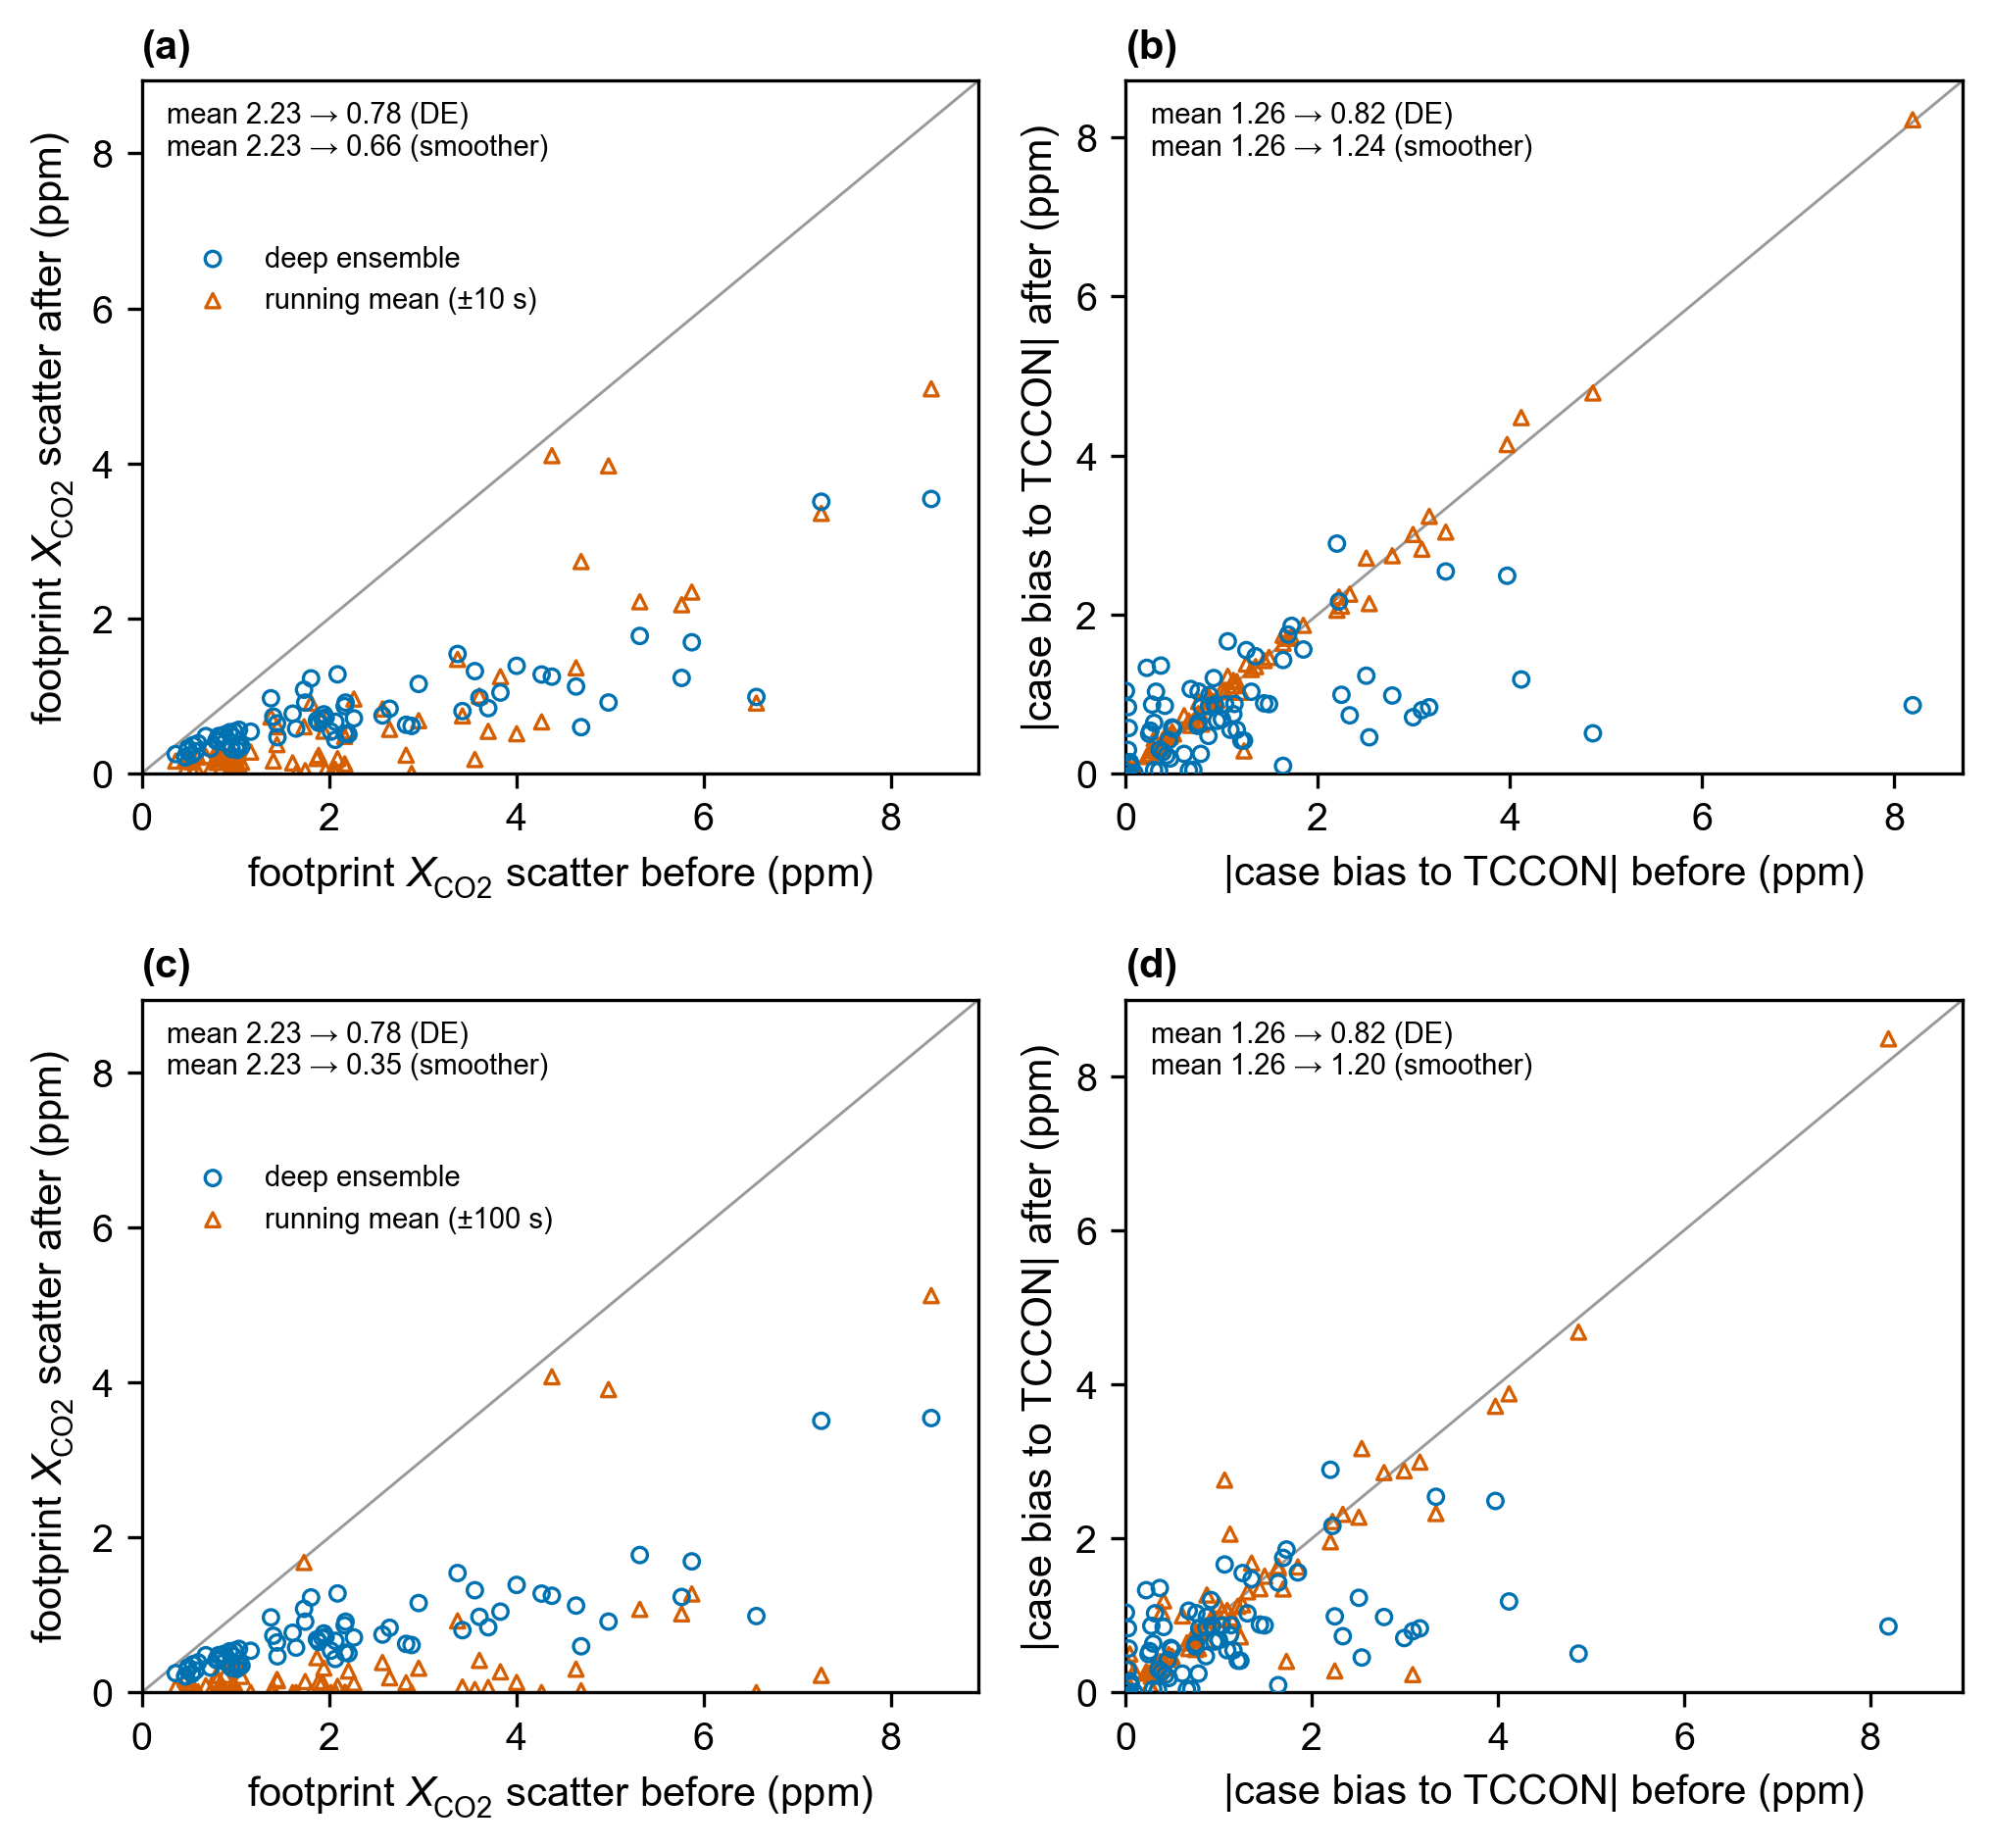
\includegraphics[width=0.8\textwidth]{figures/figE1_smoother_windows.png}
\caption{Feature-free smoother null: footprint-scatter collapse and TCCON station-day bias for orbit-local running-mean smoothers of half-width $\pm$10, $\pm$30, and $\pm$100 s beside the deep ensemble, under identical footprints, guards, and TCCON chain (windows not shown in main-text Fig.~\ref{fig:smoother_null}).}
\label{app-fig:smoother_null_full}
\end{figure}



\subsection{Negative controls}
\label{app:neg-control}



\begin{figure}[t]
\centering
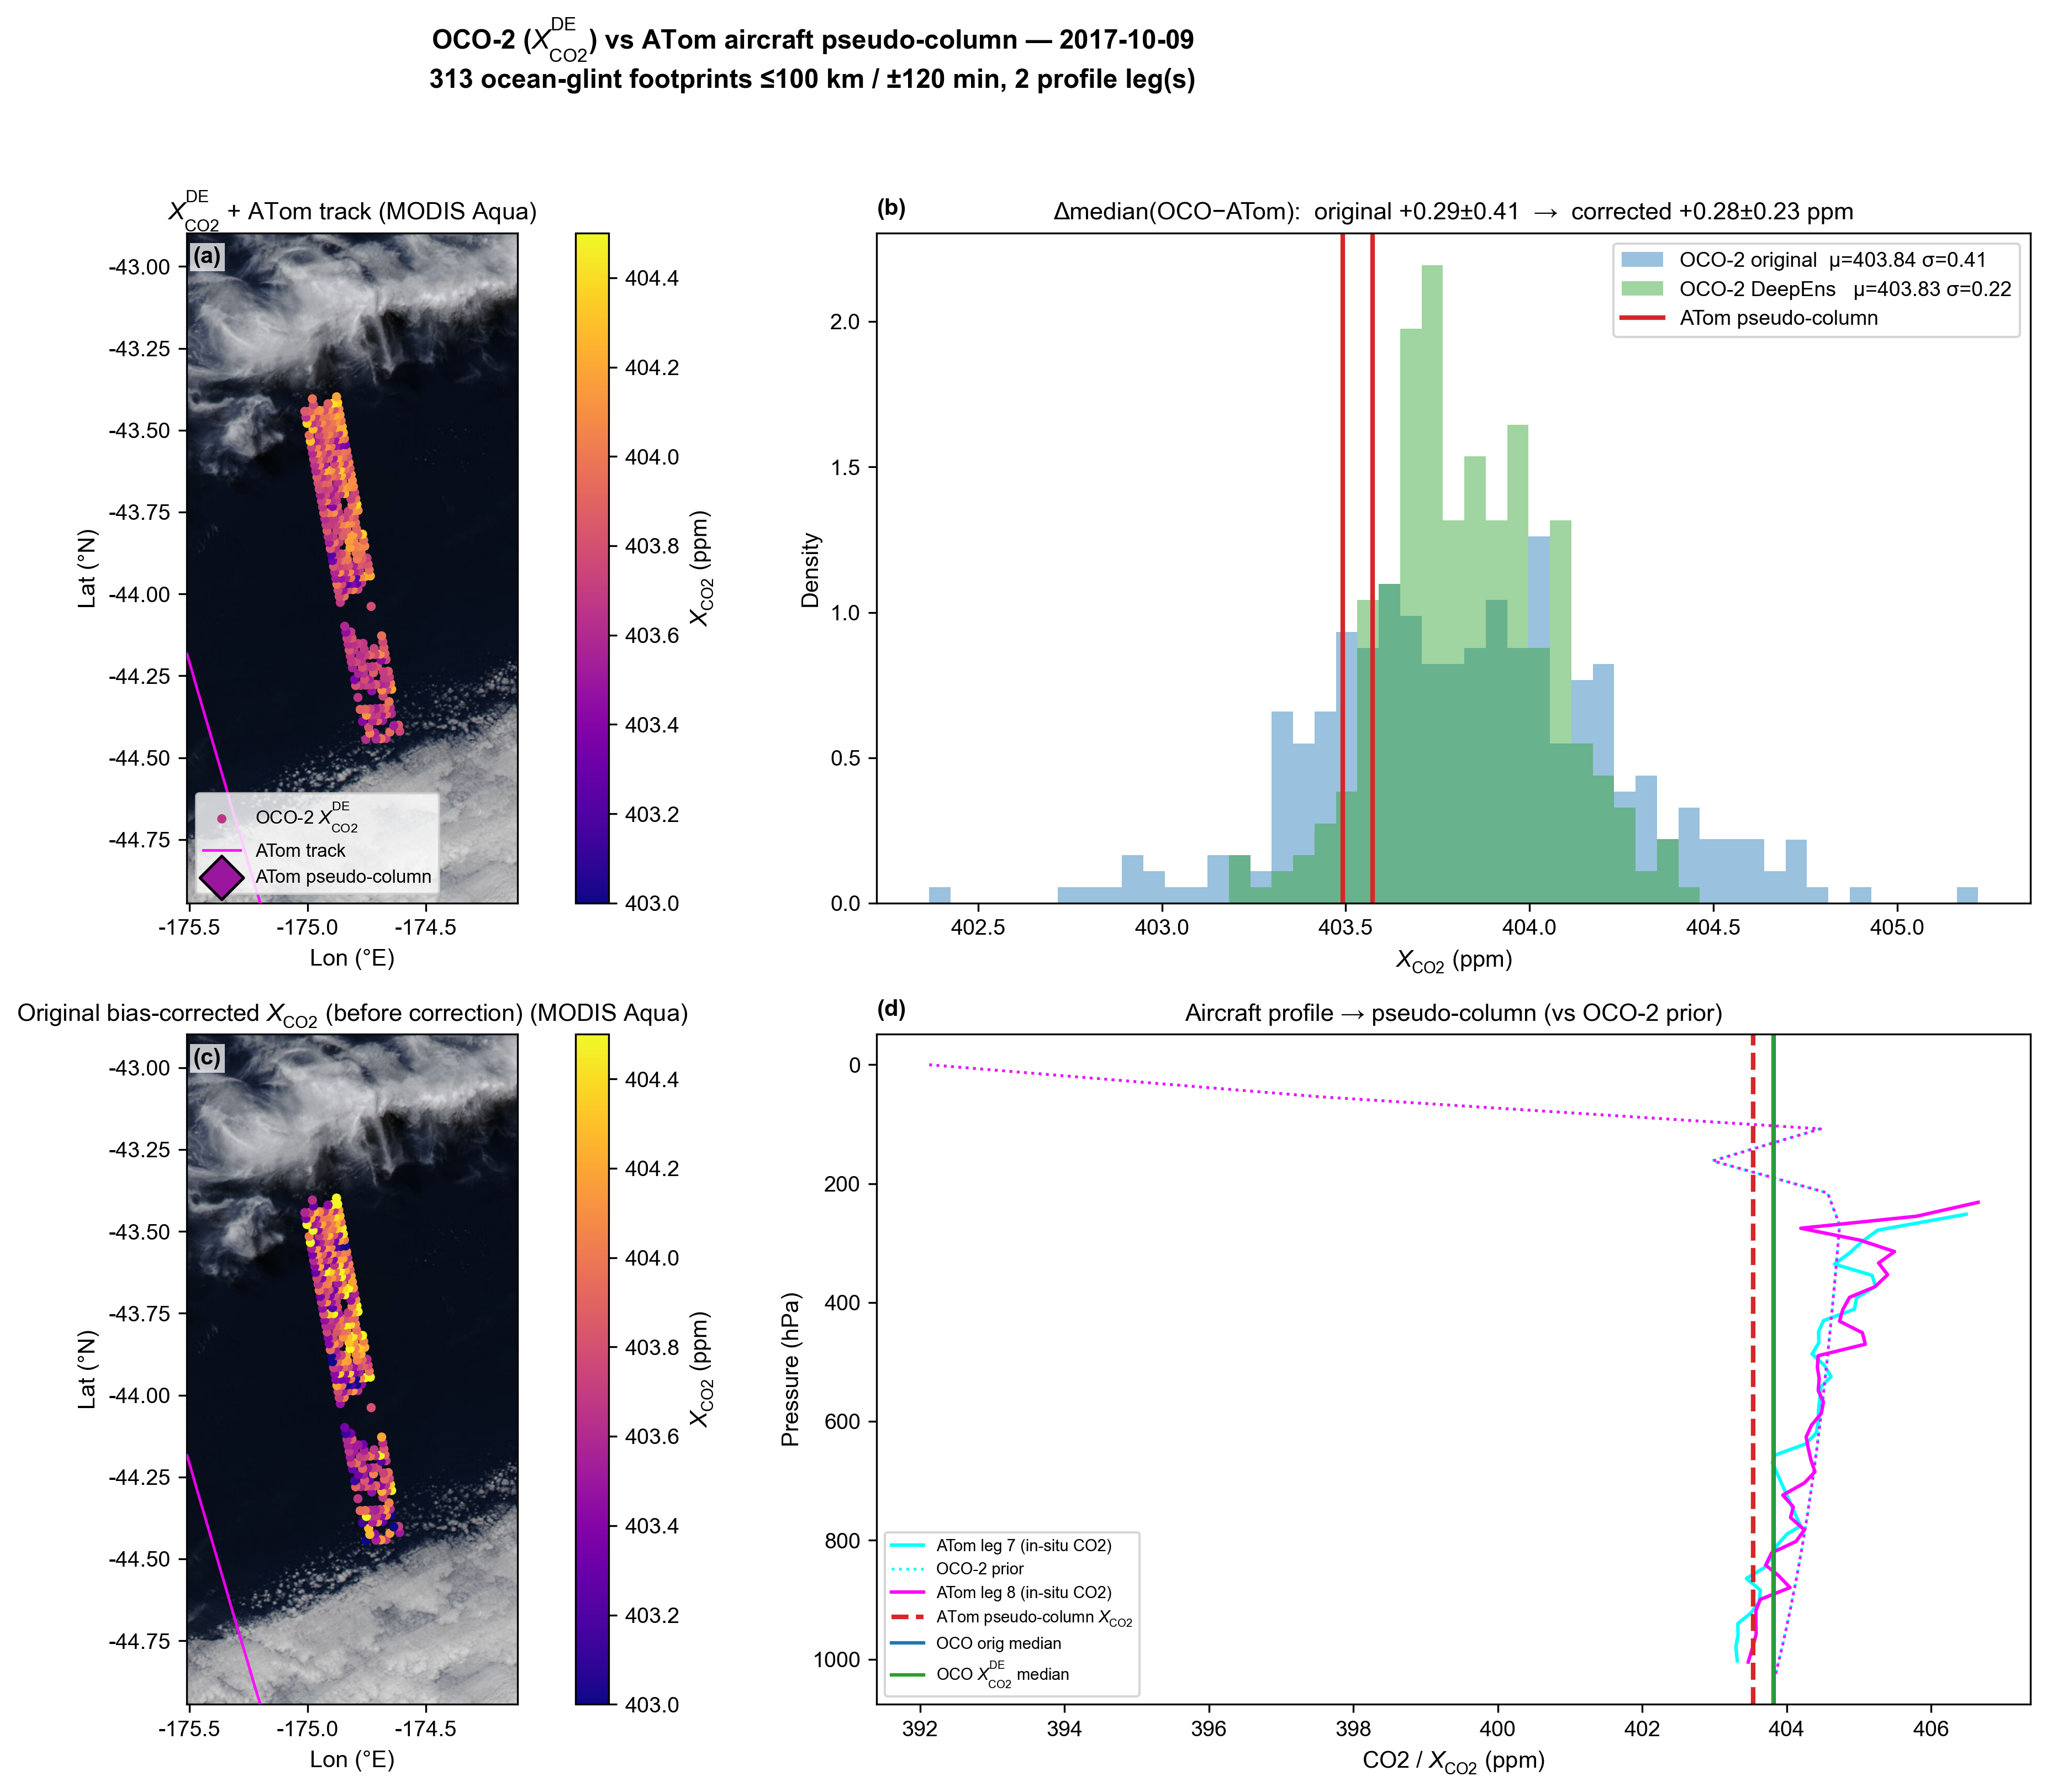
\includegraphics[width=0.8\textwidth]{figures/figE2_atom_farcloud_control.png}
\caption{ATom far-cloud negative control, 9 October 2017 (313 ocean-glint footprints within 100 km / ±120 min of two profile legs; median nearest-cloud distance 18 km): corrected and original \xco maps over the coincident MODIS Aqua true-colour scene (local day 8 October 2017 — the overpass crosses the antimeridian, where the imagery date is the local day) with the flight track, footprint distributions against the ATom pseudo-column, and the aircraft profiles with the OCO-2 prior.}
\label{app-fig:atom_far_cld}
\end{figure}


\begin{figure}[t]
\centering
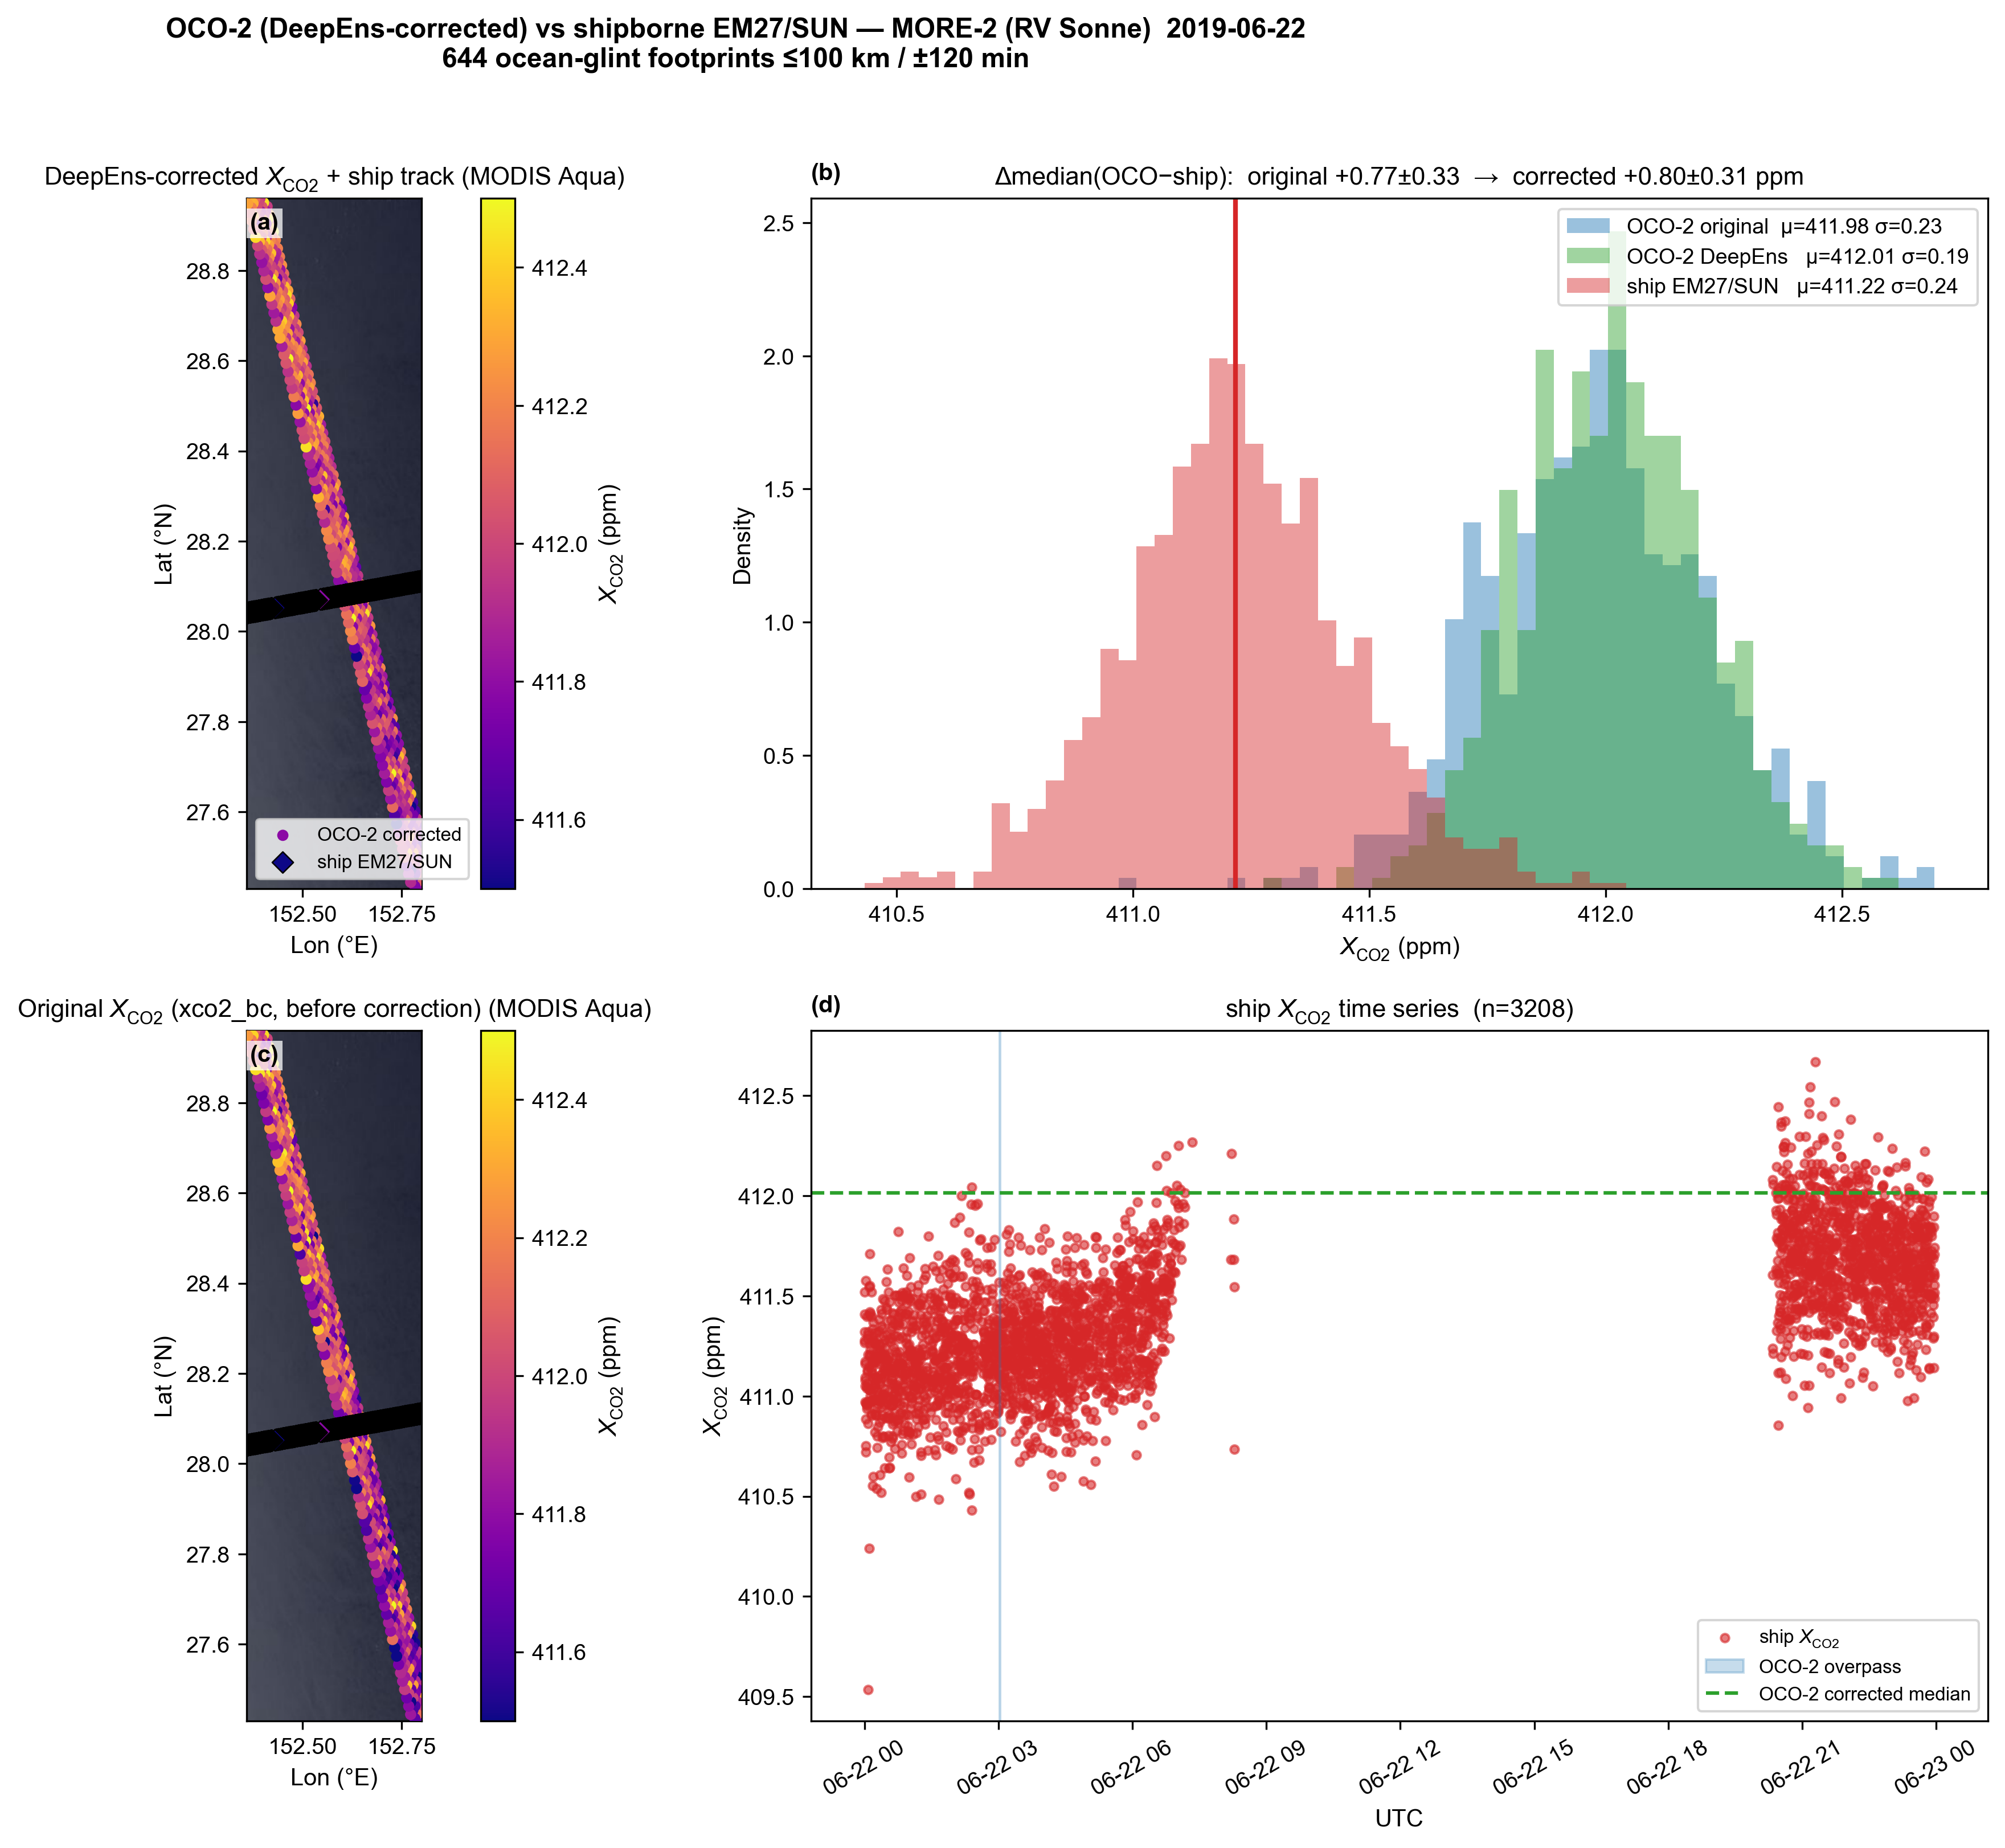
\includegraphics[width=0.8\textwidth]{figures/figE3_ship_clearday_control.png}
\caption{Shipborne clear-day negative control, 22 June 2019 (R/V Sonne EM27/SUN; 1 of 460 footprints within 10 km of cloud): same construction as Fig. E2 against the shipborne column, with the \xcoship time series around the overpass.}
\label{app-fig:ship_far_cld}
\end{figure}





\subsection{Failure cases analysis}
\label{app:tccon-failure}


\FloatBarrier


%\noappendix       %% use this to mark the end of the appendix section. Otherwise the figures might be numbered incorrectly (e.g. 10 instead of 1).

%% Regarding figures and tables in appendices, the following two options are possible depending on your general handling of figures and tables in the manuscript environment:

%% Option 1: If you sorted all figures and tables into the sections of the text, please also sort the appendix figures and appendix tables into the respective appendix sections.
%% They will be correctly named automatically.

%% Option 2: If you put all figures after the reference list, please insert appendix tables and figures after the normal tables and figures.
%% To rename them correctly to A1, A2, etc., please add the following commands in front of them:

  %% needs to be added in front of appendix figures

  %% needs to be added in front of appendix tables

%% Please add \clearpage between each table and/or figure. Further guidelines on figures and tables can be found below.